\documentclass[1p]{elsarticle_modified}
%\bibliographystyle{elsarticle-num}

%\usepackage[colorlinks]{hyperref}
%\usepackage{abbrmath_seonhwa} %\Abb, \Ascr, \Acal ,\Abf, \Afrak
\usepackage{amsfonts}
\usepackage{amssymb}
\usepackage{amsmath}
\usepackage{amsthm}
\usepackage{scalefnt}
\usepackage{amsbsy}
\usepackage{kotex}
\usepackage{caption}
\usepackage{subfig}
\usepackage{color}
\usepackage{graphicx}
\usepackage{xcolor} %% white, black, red, green, blue, cyan, magenta, yellow
\usepackage{float}
\usepackage{setspace}
\usepackage{hyperref}

\usepackage{tikz}
\usetikzlibrary{arrows}

\usepackage{multirow}
\usepackage{array} % fixed length table
\usepackage{hhline}

%%%%%%%%%%%%%%%%%%%%%
\makeatletter
\renewcommand*\env@matrix[1][\arraystretch]{%
	\edef\arraystretch{#1}%
	\hskip -\arraycolsep
	\let\@ifnextchar\new@ifnextchar
	\array{*\c@MaxMatrixCols c}}
\makeatother %https://tex.stackexchange.com/questions/14071/how-can-i-increase-the-line-spacing-in-a-matrix
%%%%%%%%%%%%%%%

\usepackage[normalem]{ulem}

\newcommand{\msout}[1]{\ifmmode\text{\sout{\ensuremath{#1}}}\else\sout{#1}\fi}
%SOURCE: \msout is \stkout macro in https://tex.stackexchange.com/questions/20609/strikeout-in-math-mode

\newcommand{\cancel}[1]{
	\ifmmode
	{\color{red}\msout{#1}}
	\else
	{\color{red}\sout{#1}}
	\fi
}

\newcommand{\add}[1]{
	{\color{blue}\uwave{#1}}
}

\newcommand{\replace}[2]{
	\ifmmode
	{\color{red}\msout{#1}}{\color{blue}\uwave{#2}}
	\else
	{\color{red}\sout{#1}}{\color{blue}\uwave{#2}}
	\fi
}

\newcommand{\Sol}{\mathcal{S}} %segment
\newcommand{\D}{D} %diagram
\newcommand{\A}{\mathcal{A}} %arc


%%%%%%%%%%%%%%%%%%%%%%%%%%%%%5 test

\def\sl{\operatorname{\textup{SL}}(2,\Cbb)}
\def\psl{\operatorname{\textup{PSL}}(2,\Cbb)}
\def\quan{\mkern 1mu \triangleright \mkern 1mu}

\theoremstyle{definition}
\newtheorem{thm}{Theorem}[section]
\newtheorem{prop}[thm]{Proposition}
\newtheorem{lem}[thm]{Lemma}
\newtheorem{ques}[thm]{Question}
\newtheorem{cor}[thm]{Corollary}
\newtheorem{defn}[thm]{Definition}
\newtheorem{exam}[thm]{Example}
\newtheorem{rmk}[thm]{Remark}
\newtheorem{alg}[thm]{Algorithm}

\newcommand{\I}{\sqrt{-1}}
\begin{document}

%\begin{frontmatter}
%
%\title{Boundary parabolic representations of knots up to 8 crossings}
%
%%% Group authors per affiliation:
%\author{Yunhi Cho} 
%\address{Department of Mathematics, University of Seoul, Seoul, Korea}
%\ead{yhcho@uos.ac.kr}
%
%
%\author{Seonhwa Kim} %\fnref{s_kim}}
%\address{Center for Geometry and Physics, Institute for Basic Science, Pohang, 37673, Korea}
%\ead{ryeona17@ibs.re.kr}
%
%\author{Hyuk Kim}
%\address{Department of Mathematical Sciences, Seoul National University, Seoul 08826, Korea}
%\ead{hyukkim@snu.ac.kr}
%
%\author{Seokbeom Yoon}
%\address{Department of Mathematical Sciences, Seoul National University, Seoul, 08826,  Korea}
%\ead{sbyoon15@snu.ac.kr}
%
%\begin{abstract}
%We find all boundary parabolic representation of knots up to 8 crossings.
%
%\end{abstract}
%\begin{keyword}
%    \MSC[2010] 57M25 
%\end{keyword}
%
%\end{frontmatter}

%\linenumbers
%\tableofcontents
%
\newcommand\colored[1]{\textcolor{white}{\rule[-0.35ex]{0.8em}{1.4ex}}\kern-0.8em\color{red} #1}%
%\newcommand\colored[1]{\textcolor{white}{ #1}\kern-2.17ex	\textcolor{white}{ #1}\kern-1.81ex	\textcolor{white}{ #1}\kern-2.15ex\color{red}#1	}

{\Large $\underline{12a_{0788}~(K12a_{0788})}$}

\setlength{\tabcolsep}{10pt}
\renewcommand{\arraystretch}{1.6}
\vspace{1cm}\begin{tabular}{m{100pt}>{\centering\arraybackslash}m{274pt}}
\multirow{5}{120pt}{
	\centering
	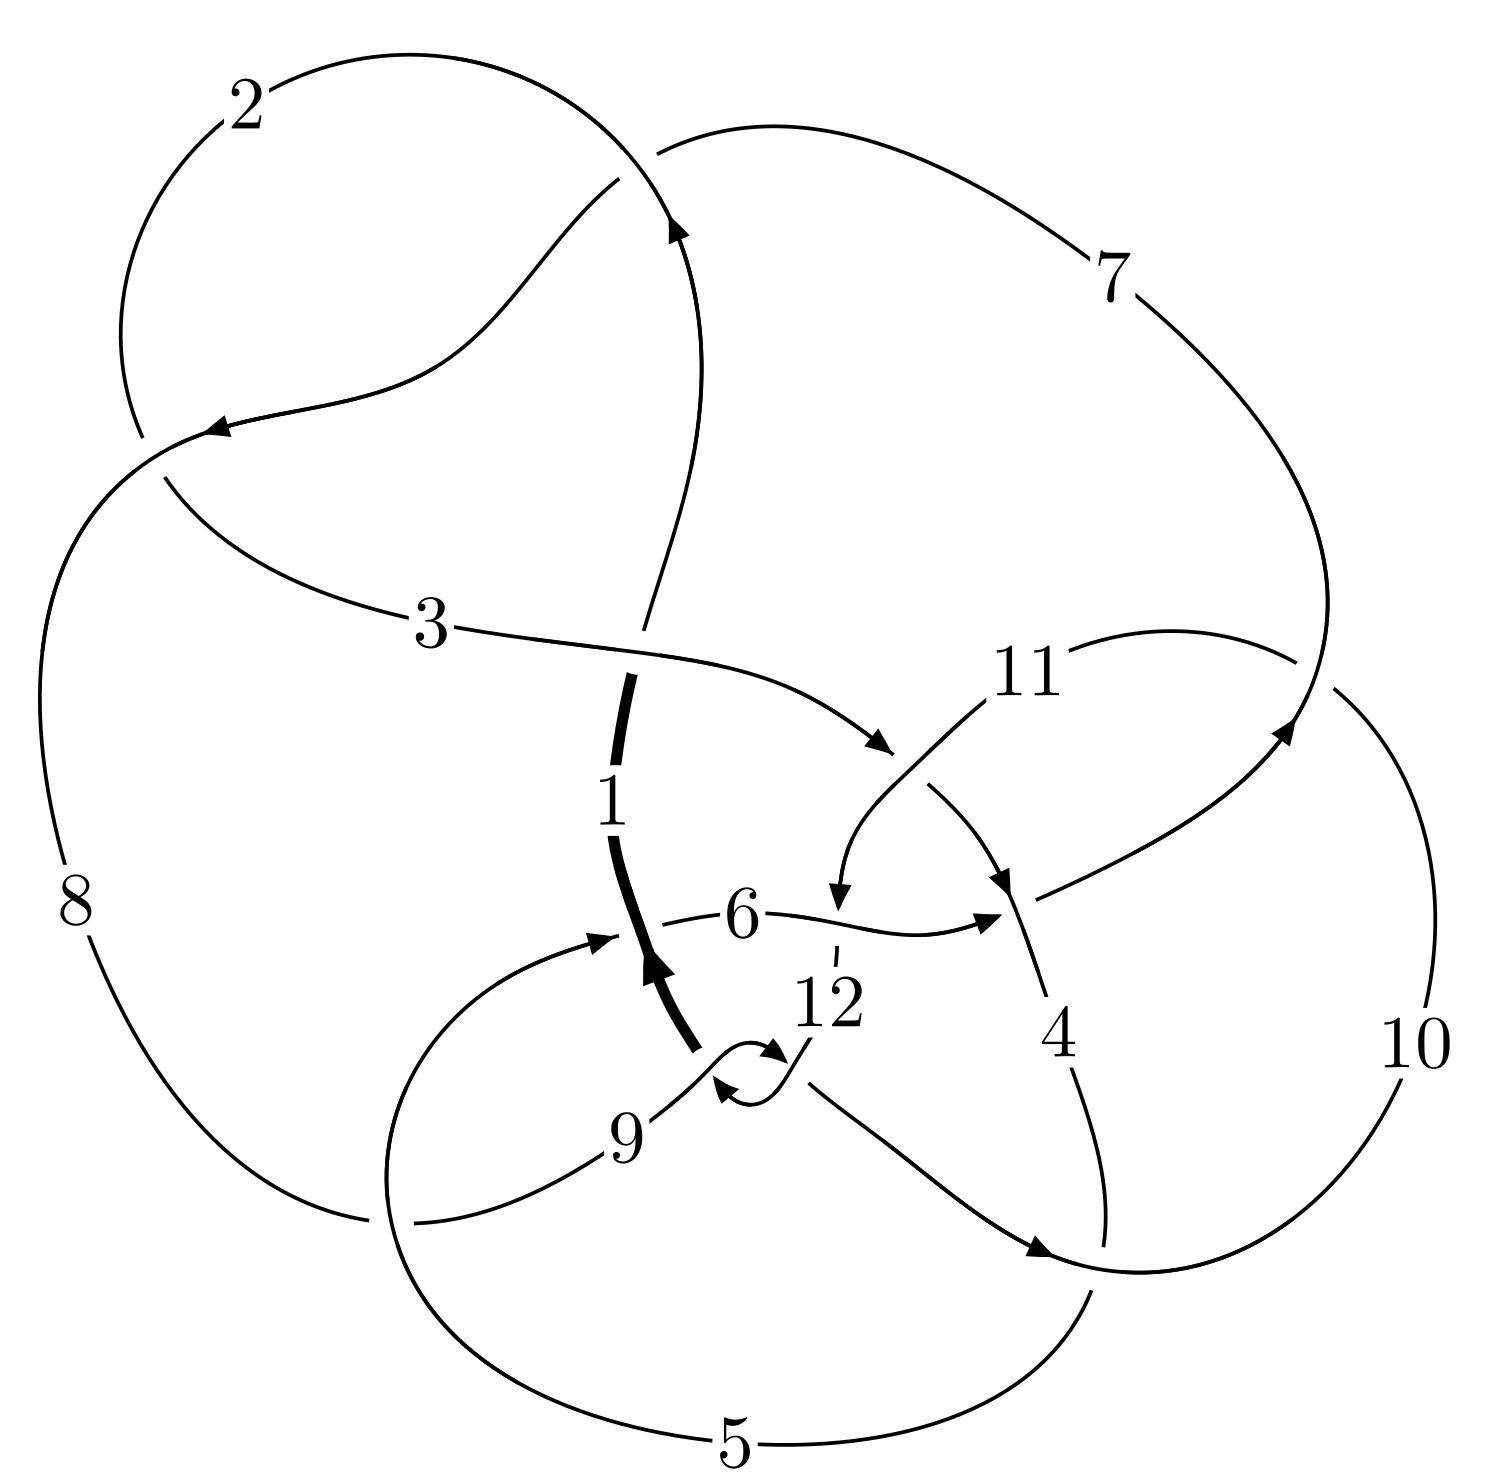
\includegraphics[width=112pt]{../../../GIT/diagram.site/Diagrams/png/1589_12a_0788.png}\\
\ \ \ A knot diagram\footnotemark}&
\allowdisplaybreaks
\textbf{Linearized knot diagam} \\
\cline{2-2}
 &
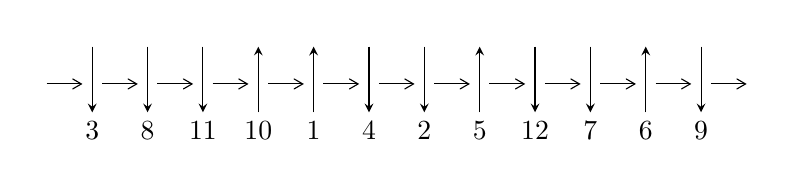
\begin{tikzpicture}[x=20pt, y=17pt]
	% nodes
	\node (C0) at (0, 0) {};
	\node (C1) at (1, 0) {};
	\node (C1U) at (1, +1) {};
	\node (C1D) at (1, -1) {3};

	\node (C2) at (2, 0) {};
	\node (C2U) at (2, +1) {};
	\node (C2D) at (2, -1) {8};

	\node (C3) at (3, 0) {};
	\node (C3U) at (3, +1) {};
	\node (C3D) at (3, -1) {11};

	\node (C4) at (4, 0) {};
	\node (C4U) at (4, +1) {};
	\node (C4D) at (4, -1) {10};

	\node (C5) at (5, 0) {};
	\node (C5U) at (5, +1) {};
	\node (C5D) at (5, -1) {1};

	\node (C6) at (6, 0) {};
	\node (C6U) at (6, +1) {};
	\node (C6D) at (6, -1) {4};

	\node (C7) at (7, 0) {};
	\node (C7U) at (7, +1) {};
	\node (C7D) at (7, -1) {2};

	\node (C8) at (8, 0) {};
	\node (C8U) at (8, +1) {};
	\node (C8D) at (8, -1) {5};

	\node (C9) at (9, 0) {};
	\node (C9U) at (9, +1) {};
	\node (C9D) at (9, -1) {12};

	\node (C10) at (10, 0) {};
	\node (C10U) at (10, +1) {};
	\node (C10D) at (10, -1) {7};

	\node (C11) at (11, 0) {};
	\node (C11U) at (11, +1) {};
	\node (C11D) at (11, -1) {6};

	\node (C12) at (12, 0) {};
	\node (C12U) at (12, +1) {};
	\node (C12D) at (12, -1) {9};
	\node (C13) at (13, 0) {};

	% arrows
	\draw[->,>={angle 60}]
	(C0) edge (C1) (C1) edge (C2) (C2) edge (C3) (C3) edge (C4) (C4) edge (C5) (C5) edge (C6) (C6) edge (C7) (C7) edge (C8) (C8) edge (C9) (C9) edge (C10) (C10) edge (C11) (C11) edge (C12) (C12) edge (C13) ;	\draw[->,>=stealth]
	(C1U) edge (C1D) (C2U) edge (C2D) (C3U) edge (C3D) (C4D) edge (C4U) (C5D) edge (C5U) (C6U) edge (C6D) (C7U) edge (C7D) (C8D) edge (C8U) (C9U) edge (C9D) (C10U) edge (C10D) (C11D) edge (C11U) (C12U) edge (C12D) ;
	\end{tikzpicture} \\
\hhline{~~} \\& 
\textbf{Solving Sequence} \\ \cline{2-2} 
 &
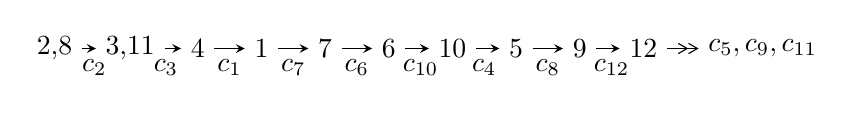
\begin{tikzpicture}[x=23pt, y=7pt]
	% node
	\node (A0) at (-1/8, 0) {2,8};
	\node (A1) at (17/16, 0) {3,11};
	\node (A2) at (17/8, 0) {4};
	\node (A3) at (25/8, 0) {1};
	\node (A4) at (33/8, 0) {7};
	\node (A5) at (41/8, 0) {6};
	\node (A6) at (49/8, 0) {10};
	\node (A7) at (57/8, 0) {5};
	\node (A8) at (65/8, 0) {9};
	\node (A9) at (73/8, 0) {12};
	\node (C1) at (1/2, -1) {$c_{2}$};
	\node (C2) at (13/8, -1) {$c_{3}$};
	\node (C3) at (21/8, -1) {$c_{1}$};
	\node (C4) at (29/8, -1) {$c_{7}$};
	\node (C5) at (37/8, -1) {$c_{6}$};
	\node (C6) at (45/8, -1) {$c_{10}$};
	\node (C7) at (53/8, -1) {$c_{4}$};
	\node (C8) at (61/8, -1) {$c_{8}$};
	\node (C9) at (69/8, -1) {$c_{12}$};
	\node (A10) at (11, 0) {$c_{5},c_{9},c_{11}$};

	% edge
	\draw[->,>=stealth]	
	(A0) edge (A1) (A1) edge (A2) (A2) edge (A3) (A3) edge (A4) (A4) edge (A5) (A5) edge (A6) (A6) edge (A7) (A7) edge (A8) (A8) edge (A9) ;
	\draw[->>,>={angle 60}]	
	(A9) edge (A10);
\end{tikzpicture} \\ 

\end{tabular} \\

\footnotetext{
The image of knot diagram is generated by the software ``\textbf{Draw programme}" developed by Andrew Bartholomew(\url{http://www.layer8.co.uk/maths/draw/index.htm\#Running-draw}), where we modified some parts for our purpose(\url{https://github.com/CATsTAILs/LinksPainter}).
}\phantom \\ \newline 
\centering \textbf{Ideals for irreducible components\footnotemark of $X_{\text{par}}$} 
 
\begin{align*}
I^u_{1}&=\langle 
-7.48372\times10^{14} u^{59}-1.40888\times10^{16} u^{58}+\cdots+1.09132\times10^{11} b+1.02559\times10^{18},\\
\phantom{I^u_{1}}&\phantom{= \langle  }-1.00155\times10^{15} u^{59}-1.85343\times10^{16} u^{58}+\cdots+2.18264\times10^{11} a+9.84042\times10^{17},\\
\phantom{I^u_{1}}&\phantom{= \langle  }u^{60}+20 u^{59}+\cdots-27648 u-2048\rangle \\
I^u_{2}&=\langle 
1.40209\times10^{270} a^{21} u^{5}+1.35540\times10^{271} a^{20} u^{5}+\cdots-1.14418\times10^{274} a-7.36836\times10^{272},\\
\phantom{I^u_{2}}&\phantom{= \langle  }-3 a^{21} u^5+2 a^{20} u^5+\cdots+91 a+98,\;u^6- u^5- u^4+2 u^3- u+1\rangle \\
I^u_{3}&=\langle 
-2121378380 u^{44}+1708716794 u^{43}+\cdots+57230447 b-2318247446,\\
\phantom{I^u_{3}}&\phantom{= \langle  }-2318247446 u^{44}+2515116512 u^{43}+\cdots+57230447 a-1658167052,\;u^{45}-2 u^{44}+\cdots+2 u-1\rangle \\
I^u_{4}&=\langle 
b-1,\;a- u-1,\;u^2+u+1\rangle \\
\\
\end{align*}
\raggedright * 4 irreducible components of $\dim_{\mathbb{C}}=0$, with total 239 representations.\\
\footnotetext{All coefficients of polynomials are rational numbers. But the coefficients are sometimes approximated in decimal forms when there is not enough margin.}
\newpage
\renewcommand{\arraystretch}{1}
\centering \section*{I. $I^u_{1}= \langle -7.48\times10^{14} u^{59}-1.41\times10^{16} u^{58}+\cdots+1.09\times10^{11} b+1.03\times10^{18},\;-1.00\times10^{15} u^{59}-1.85\times10^{16} u^{58}+\cdots+2.18\times10^{11} a+9.84\times10^{17},\;u^{60}+20 u^{59}+\cdots-27648 u-2048 \rangle$}
\flushleft \textbf{(i) Arc colorings}\\
\begin{tabular}{m{7pt} m{180pt} m{7pt} m{180pt} }
\flushright $a_{2}=$&$\begin{pmatrix}1\\0\end{pmatrix}$ \\
\flushright $a_{8}=$&$\begin{pmatrix}0\\u\end{pmatrix}$ \\
\flushright $a_{3}=$&$\begin{pmatrix}1\\u^2\end{pmatrix}$ \\
\flushright $a_{11}=$&$\begin{pmatrix}4588.72 u^{59}+84916.9 u^{58}+\cdots-6.02606\times10^{7} u-4.50849\times10^{6}\\6857.49 u^{59}+129098. u^{58}+\cdots-1.22360\times10^{8} u-9.39770\times10^{6}\end{pmatrix}$ \\
\flushright $a_{4}=$&$\begin{pmatrix}250.351 u^{59}+5495.68 u^{58}+\cdots-1.44691\times10^{7} u-1.15895\times10^{6}\\-488.667 u^{59}-8145.45 u^{58}+\cdots-5.76275\times10^{6} u-512719.\end{pmatrix}$ \\
\flushright $a_{1}=$&$\begin{pmatrix}- u^2+1\\- u^4\end{pmatrix}$ \\
\flushright $a_{7}=$&$\begin{pmatrix}u\\u\end{pmatrix}$ \\
\flushright $a_{6}=$&$\begin{pmatrix}1325.73 u^{59}+24882.4 u^{58}+\cdots-2.45048\times10^{7} u-1.89309\times10^{6}\\1986.08 u^{59}+36969.0 u^{58}+\cdots-3.14103\times10^{7} u-2.40620\times10^{6}\end{pmatrix}$ \\
\flushright $a_{10}=$&$\begin{pmatrix}3514.76 u^{59}+67929.5 u^{58}+\cdots-8.86252\times10^{7} u-6.95375\times10^{6}\\5783.53 u^{59}+112111. u^{58}+\cdots-1.50725\times10^{8} u-1.18430\times10^{7}\end{pmatrix}$ \\
\flushright $a_{5}=$&$\begin{pmatrix}238.438 u^{59}+3950.12 u^{58}+\cdots+5.58629\times10^{6} u+496872.\\-218.983 u^{59}-5479.84 u^{58}+\cdots+2.60400\times10^{7} u+2.13851\times10^{6}\end{pmatrix}$ \\
\flushright $a_{9}=$&$\begin{pmatrix}-129.456 u^{59}-2345.21 u^{58}+\cdots+2.05852\times10^{6} u+170613.\\-1118.08 u^{59}-21011.6 u^{58}+\cdots+2.28800\times10^{7} u+1.79800\times10^{6}\end{pmatrix}$ \\
\flushright $a_{12}=$&$\begin{pmatrix}-1645.01 u^{59}-30594.3 u^{58}+\cdots+2.26877\times10^{7} u+1.70023\times10^{6}\\-3467.72 u^{59}-64602.7 u^{58}+\cdots+5.02340\times10^{7} u+3.79319\times10^{6}\end{pmatrix}$\\&\end{tabular}
\flushleft \textbf{(ii) Obstruction class $= -1$}\\~\\
\flushleft \textbf{(iii) Cusp Shapes $= \frac{36746774069337}{13641503552} u^{59}+\frac{1434372875041167}{27283007104} u^{58}+\cdots-\frac{15915677814015894}{213148493} u-\frac{1254542070951070}{213148493}$}\\~\\
\newpage\renewcommand{\arraystretch}{1}
\flushleft \textbf{(iv) u-Polynomials at the component}\newline \\
\begin{tabular}{m{50pt}|m{274pt}}
Crossings & \hspace{64pt}u-Polynomials at each crossing \\
\hline $$\begin{aligned}c_{1}\end{aligned}$$&$\begin{aligned}
&u^{60}+34 u^{59}+\cdots+13631488 u+4194304
\end{aligned}$\\
\hline $$\begin{aligned}c_{2},c_{7}\end{aligned}$$&$\begin{aligned}
&u^{60}-20 u^{59}+\cdots+27648 u-2048
\end{aligned}$\\
\hline $$\begin{aligned}c_{3},c_{10}\end{aligned}$$&$\begin{aligned}
&u^{60}+2 u^{59}+\cdots+4 u-1
\end{aligned}$\\
\hline $$\begin{aligned}c_{4},c_{11}\end{aligned}$$&$\begin{aligned}
&u^{60}+7 u^{58}+\cdots-2 u-21
\end{aligned}$\\
\hline $$\begin{aligned}c_{5},c_{8}\end{aligned}$$&$\begin{aligned}
&u^{60}+4 u^{59}+\cdots+23 u-1
\end{aligned}$\\
\hline $$\begin{aligned}c_{6}\end{aligned}$$&$\begin{aligned}
&u^{60}-41 u^{59}+\cdots-416 u+64
\end{aligned}$\\
\hline $$\begin{aligned}c_{9},c_{12}\end{aligned}$$&$\begin{aligned}
&u^{60}-21 u^{59}+\cdots-66560 u+4096
\end{aligned}$\\
\hline
\end{tabular}\\~\\
\newpage\renewcommand{\arraystretch}{1}
\flushleft \textbf{(v) Riley Polynomials at the component}\newline \\
\begin{tabular}{m{50pt}|m{274pt}}
Crossings & \hspace{64pt}Riley Polynomials at each crossing \\
\hline $$\begin{aligned}c_{1}\end{aligned}$$&$\begin{aligned}
&y^{60}-14 y^{59}+\cdots+355142255771648 y+17592186044416
\end{aligned}$\\
\hline $$\begin{aligned}c_{2},c_{7}\end{aligned}$$&$\begin{aligned}
&y^{60}-34 y^{59}+\cdots-13631488 y+4194304
\end{aligned}$\\
\hline $$\begin{aligned}c_{3},c_{10}\end{aligned}$$&$\begin{aligned}
&y^{60}+10 y^{59}+\cdots+18 y+1
\end{aligned}$\\
\hline $$\begin{aligned}c_{4},c_{11}\end{aligned}$$&$\begin{aligned}
&y^{60}+14 y^{59}+\cdots+2768 y+441
\end{aligned}$\\
\hline $$\begin{aligned}c_{5},c_{8}\end{aligned}$$&$\begin{aligned}
&y^{60}-30 y^{59}+\cdots-629 y+1
\end{aligned}$\\
\hline $$\begin{aligned}c_{6}\end{aligned}$$&$\begin{aligned}
&y^{60}-7 y^{59}+\cdots-119808 y+4096
\end{aligned}$\\
\hline $$\begin{aligned}c_{9},c_{12}\end{aligned}$$&$\begin{aligned}
&y^{60}+29 y^{59}+\cdots+103809024 y+16777216
\end{aligned}$\\
\hline
\end{tabular}\\~\\
\newpage\flushleft \textbf{(vi) Complex Volumes and Cusp Shapes}
$$\begin{array}{c|c|c}  
\text{Solutions to }I^u_{1}& \I (\text{vol} + \sqrt{-1}CS) & \text{Cusp shape}\\
 \hline 
\begin{aligned}
u &= -0.333620 + 0.934820 I \\
a &= \phantom{-}0.674936 + 1.218260 I \\
b &= \phantom{-}1.364030 - 0.224508 I\end{aligned}
 & \phantom{-}2.2681 - 15.8299 I & \phantom{-0.000000 } 0 \\ \hline\begin{aligned}
u &= -0.333620 - 0.934820 I \\
a &= \phantom{-}0.674936 - 1.218260 I \\
b &= \phantom{-}1.364030 + 0.224508 I\end{aligned}
 & \phantom{-}2.2681 + 15.8299 I & \phantom{-0.000000 } 0 \\ \hline\begin{aligned}
u &= -0.313471 + 0.961263 I \\
a &= -0.601185 - 1.165240 I \\
b &= -1.308550 + 0.212628 I\end{aligned}
 & -1.49873 - 9.71181 I & \phantom{-0.000000 } 0 \\ \hline\begin{aligned}
u &= -0.313471 - 0.961263 I \\
a &= -0.601185 + 1.165240 I \\
b &= -1.308550 - 0.212628 I\end{aligned}
 & -1.49873 + 9.71181 I & \phantom{-0.000000 } 0 \\ \hline\begin{aligned}
u &= \phantom{-}0.944174 + 0.249030 I \\
a &= -0.081713 + 0.383364 I \\
b &= \phantom{-}0.172621 - 0.341613 I\end{aligned}
 & -0.507559 - 0.907664 I & \phantom{-0.000000 } 0 \\ \hline\begin{aligned}
u &= \phantom{-}0.944174 - 0.249030 I \\
a &= -0.081713 - 0.383364 I \\
b &= \phantom{-}0.172621 + 0.341613 I\end{aligned}
 & -0.507559 + 0.907664 I & \phantom{-0.000000 } 0 \\ \hline\begin{aligned}
u &= -0.697333 + 0.759169 I \\
a &= \phantom{-}0.809520 + 0.902124 I \\
b &= \phantom{-}1.249370 + 0.014518 I\end{aligned}
 & \phantom{-}3.10973 + 0.23218 I & \phantom{-0.000000 } 0 \\ \hline\begin{aligned}
u &= -0.697333 - 0.759169 I \\
a &= \phantom{-}0.809520 - 0.902124 I \\
b &= \phantom{-}1.249370 - 0.014518 I\end{aligned}
 & \phantom{-}3.10973 - 0.23218 I & \phantom{-0.000000 } 0 \\ \hline\begin{aligned}
u &= -0.145685 + 0.934102 I \\
a &= -0.001093 - 0.424826 I \\
b &= -0.396990 - 0.060870 I\end{aligned}
 & \phantom{-}0.27991 - 2.30790 I & \phantom{-0.000000 } 0 \\ \hline\begin{aligned}
u &= -0.145685 - 0.934102 I \\
a &= -0.001093 + 0.424826 I \\
b &= -0.396990 + 0.060870 I\end{aligned}
 & \phantom{-}0.27991 + 2.30790 I & \phantom{-0.000000 } 0\\
 \hline 
 \end{array}$$\newpage$$\begin{array}{c|c|c}  
\text{Solutions to }I^u_{1}& \I (\text{vol} + \sqrt{-1}CS) & \text{Cusp shape}\\
 \hline 
\begin{aligned}
u &= -0.780293 + 0.715158 I \\
a &= -0.08445 - 1.54692 I \\
b &= -1.17219 - 1.14665 I\end{aligned}
 & \phantom{-}7.75560 + 1.60562 I & \phantom{-0.000000 } 0 \\ \hline\begin{aligned}
u &= -0.780293 - 0.715158 I \\
a &= -0.08445 + 1.54692 I \\
b &= -1.17219 + 1.14665 I\end{aligned}
 & \phantom{-}7.75560 - 1.60562 I & \phantom{-0.000000 } 0 \\ \hline\begin{aligned}
u &= -0.187677 + 0.905842 I \\
a &= \phantom{-}0.367951 + 1.279140 I \\
b &= \phantom{-}1.227760 - 0.093240 I\end{aligned}
 & \phantom{-}4.33323 - 3.97038 I & \phantom{-0.000000 } 0 \\ \hline\begin{aligned}
u &= -0.187677 - 0.905842 I \\
a &= \phantom{-}0.367951 - 1.279140 I \\
b &= \phantom{-}1.227760 + 0.093240 I\end{aligned}
 & \phantom{-}4.33323 + 3.97038 I & \phantom{-0.000000 } 0 \\ \hline\begin{aligned}
u &= -0.303550 + 1.037960 I \\
a &= \phantom{-}0.270953 + 0.350153 I \\
b &= \phantom{-}0.445694 - 0.174951 I\end{aligned}
 & \phantom{-}2.68007 - 6.88503 I & \phantom{-0.000000 } 0 \\ \hline\begin{aligned}
u &= -0.303550 - 1.037960 I \\
a &= \phantom{-}0.270953 - 0.350153 I \\
b &= \phantom{-}0.445694 + 0.174951 I\end{aligned}
 & \phantom{-}2.68007 + 6.88503 I & \phantom{-0.000000 } 0 \\ \hline\begin{aligned}
u &= -0.848038 + 0.707790 I \\
a &= -1.104920 - 0.731601 I \\
b &= -1.45484 + 0.16163 I\end{aligned}
 & \phantom{-}7.56196 + 3.77097 I & \phantom{-0.000000 } 0 \\ \hline\begin{aligned}
u &= -0.848038 - 0.707790 I \\
a &= -1.104920 + 0.731601 I \\
b &= -1.45484 - 0.16163 I\end{aligned}
 & \phantom{-}7.56196 - 3.77097 I & \phantom{-0.000000 } 0 \\ \hline\begin{aligned}
u &= -1.070680 + 0.508372 I \\
a &= \phantom{-}1.26524 + 0.88222 I \\
b &= \phantom{-}1.80317 + 0.30136 I\end{aligned}
 & \phantom{-}1.92878 + 5.49302 I & \phantom{-0.000000 } 0 \\ \hline\begin{aligned}
u &= -1.070680 - 0.508372 I \\
a &= \phantom{-}1.26524 - 0.88222 I \\
b &= \phantom{-}1.80317 - 0.30136 I\end{aligned}
 & \phantom{-}1.92878 - 5.49302 I & \phantom{-0.000000 } 0\\
 \hline 
 \end{array}$$\newpage$$\begin{array}{c|c|c}  
\text{Solutions to }I^u_{1}& \I (\text{vol} + \sqrt{-1}CS) & \text{Cusp shape}\\
 \hline 
\begin{aligned}
u &= -0.824091 + 0.858404 I \\
a &= -0.070507 - 1.171040 I \\
b &= -1.063330 - 0.904520 I\end{aligned}
 & \phantom{-}5.37941 + 11.52000 I & \phantom{-0.000000 } 0 \\ \hline\begin{aligned}
u &= -0.824091 - 0.858404 I \\
a &= -0.070507 + 1.171040 I \\
b &= -1.063330 + 0.904520 I\end{aligned}
 & \phantom{-}5.37941 - 11.52000 I & \phantom{-0.000000 } 0 \\ \hline\begin{aligned}
u &= -0.905721 + 0.787538 I \\
a &= \phantom{-}0.293055 + 1.287800 I \\
b &= \phantom{-}1.27962 + 0.93560 I\end{aligned}
 & \phantom{-}2.52360 + 5.52538 I & \phantom{-0.000000 } 0 \\ \hline\begin{aligned}
u &= -0.905721 - 0.787538 I \\
a &= \phantom{-}0.293055 - 1.287800 I \\
b &= \phantom{-}1.27962 - 0.93560 I\end{aligned}
 & \phantom{-}2.52360 - 5.52538 I & \phantom{-0.000000 } 0 \\ \hline\begin{aligned}
u &= -0.420754 + 0.679305 I \\
a &= -0.26528 - 1.64093 I \\
b &= -1.226310 - 0.510218 I\end{aligned}
 & \phantom{-}3.52442 - 0.82636 I & \phantom{-0.000000 } 0 \\ \hline\begin{aligned}
u &= -0.420754 - 0.679305 I \\
a &= -0.26528 + 1.64093 I \\
b &= -1.226310 + 0.510218 I\end{aligned}
 & \phantom{-}3.52442 + 0.82636 I & \phantom{-0.000000 } 0 \\ \hline\begin{aligned}
u &= -1.075920 + 0.562568 I \\
a &= -1.32077 - 1.35476 I \\
b &= -2.18319 - 0.71459 I\end{aligned}
 & \phantom{-}1.61159 + 5.63980 I & \phantom{-0.000000 } 0 \\ \hline\begin{aligned}
u &= -1.075920 - 0.562568 I \\
a &= -1.32077 + 1.35476 I \\
b &= -2.18319 + 0.71459 I\end{aligned}
 & \phantom{-}1.61159 - 5.63980 I & \phantom{-0.000000 } 0 \\ \hline\begin{aligned}
u &= -0.838313 + 0.884571 I \\
a &= -0.727740 - 0.574385 I \\
b &= -1.118160 + 0.162223 I\end{aligned}
 & \phantom{-}5.35357 - 5.24503 I & \phantom{-0.000000 } 0 \\ \hline\begin{aligned}
u &= -0.838313 - 0.884571 I \\
a &= -0.727740 + 0.574385 I \\
b &= -1.118160 - 0.162223 I\end{aligned}
 & \phantom{-}5.35357 + 5.24503 I & \phantom{-0.000000 } 0\\
 \hline 
 \end{array}$$\newpage$$\begin{array}{c|c|c}  
\text{Solutions to }I^u_{1}& \I (\text{vol} + \sqrt{-1}CS) & \text{Cusp shape}\\
 \hline 
\begin{aligned}
u &= \phantom{-}1.159010 + 0.393572 I \\
a &= \phantom{-}0.221908 - 0.440917 I \\
b &= -0.430725 + 0.423688 I\end{aligned}
 & \phantom{-}0.101185 - 0.165210 I & \phantom{-0.000000 } 0 \\ \hline\begin{aligned}
u &= \phantom{-}1.159010 - 0.393572 I \\
a &= \phantom{-}0.221908 + 0.440917 I \\
b &= -0.430725 - 0.423688 I\end{aligned}
 & \phantom{-}0.101185 + 0.165210 I & \phantom{-0.000000 } 0 \\ \hline\begin{aligned}
u &= -0.456971 + 0.622877 I \\
a &= -0.07193 + 1.60525 I \\
b &= \phantom{-}0.967003 + 0.778358 I\end{aligned}
 & \phantom{-}3.74351 - 1.00486 I & \phantom{-0.000000 } 0 \\ \hline\begin{aligned}
u &= -0.456971 - 0.622877 I \\
a &= -0.07193 - 1.60525 I \\
b &= \phantom{-}0.967003 - 0.778358 I\end{aligned}
 & \phantom{-}3.74351 + 1.00486 I & \phantom{-0.000000 } 0 \\ \hline\begin{aligned}
u &= -1.079430 + 0.603300 I \\
a &= \phantom{-}0.80779 + 1.26432 I \\
b &= \phantom{-}1.63471 + 0.87741 I\end{aligned}
 & \phantom{-}1.49576 + 5.38757 I & \phantom{-0.000000 } 0 \\ \hline\begin{aligned}
u &= -1.079430 - 0.603300 I \\
a &= \phantom{-}0.80779 - 1.26432 I \\
b &= \phantom{-}1.63471 - 0.87741 I\end{aligned}
 & \phantom{-}1.49576 - 5.38757 I & \phantom{-0.000000 } 0 \\ \hline\begin{aligned}
u &= \phantom{-}0.733772\phantom{ +0.000000I} \\
a &= \phantom{-}0.687778\phantom{ +0.000000I} \\
b &= -0.504672\phantom{ +0.000000I}\end{aligned}
 & -1.46322\phantom{ +0.000000I} & \phantom{-0.000000 } 0 \\ \hline\begin{aligned}
u &= \phantom{-}1.324830 + 0.182582 I \\
a &= \phantom{-}0.269732 - 0.353967 I \\
b &= -0.421977 + 0.419697 I\end{aligned}
 & -3.44520 + 12.20910 I & \phantom{-0.000000 } 0 \\ \hline\begin{aligned}
u &= \phantom{-}1.324830 - 0.182582 I \\
a &= \phantom{-}0.269732 + 0.353967 I \\
b &= -0.421977 - 0.419697 I\end{aligned}
 & -3.44520 - 12.20910 I & \phantom{-0.000000 } 0 \\ \hline\begin{aligned}
u &= -1.184740 + 0.623579 I \\
a &= \phantom{-}1.01088 + 1.65429 I \\
b &= \phantom{-}2.22921 + 1.32954 I\end{aligned}
 & -0.3203 + 21.5045 I & \phantom{-0.000000 } 0\\
 \hline 
 \end{array}$$\newpage$$\begin{array}{c|c|c}  
\text{Solutions to }I^u_{1}& \I (\text{vol} + \sqrt{-1}CS) & \text{Cusp shape}\\
 \hline 
\begin{aligned}
u &= -1.184740 - 0.623579 I \\
a &= \phantom{-}1.01088 - 1.65429 I \\
b &= \phantom{-}2.22921 - 1.32954 I\end{aligned}
 & -0.3203 - 21.5045 I & \phantom{-0.000000 } 0 \\ \hline\begin{aligned}
u &= -1.198680 + 0.625931 I \\
a &= -1.00532 - 1.57397 I \\
b &= -2.19026 - 1.25744 I\end{aligned}
 & -4.1959 + 15.4585 I & \phantom{-0.000000 } 0 \\ \hline\begin{aligned}
u &= -1.198680 - 0.625931 I \\
a &= -1.00532 + 1.57397 I \\
b &= -2.19026 + 1.25744 I\end{aligned}
 & -4.1959 - 15.4585 I & \phantom{-0.000000 } 0 \\ \hline\begin{aligned}
u &= -1.232080 + 0.594174 I \\
a &= -0.480166 - 0.705714 I \\
b &= -1.010920 - 0.584195 I\end{aligned}
 & -2.90188 + 7.84313 I & \phantom{-0.000000 } 0 \\ \hline\begin{aligned}
u &= -1.232080 - 0.594174 I \\
a &= -0.480166 + 0.705714 I \\
b &= -1.010920 + 0.584195 I\end{aligned}
 & -2.90188 - 7.84313 I & \phantom{-0.000000 } 0 \\ \hline\begin{aligned}
u &= -1.357810 + 0.168665 I \\
a &= -0.502833 + 0.534844 I \\
b &= -0.592539 + 0.811023 I\end{aligned}
 & -5.60267 + 3.59176 I & \phantom{-0.000000 } 0 \\ \hline\begin{aligned}
u &= -1.357810 - 0.168665 I \\
a &= -0.502833 - 0.534844 I \\
b &= -0.592539 - 0.811023 I\end{aligned}
 & -5.60267 - 3.59176 I & \phantom{-0.000000 } 0 \\ \hline\begin{aligned}
u &= -1.238410 + 0.587165 I \\
a &= \phantom{-}1.17216 + 1.44428 I \\
b &= \phantom{-}2.29964 + 1.10036 I\end{aligned}
 & \phantom{-}1.18187 + 9.43402 I & \phantom{-0.000000 } 0 \\ \hline\begin{aligned}
u &= -1.238410 - 0.587165 I \\
a &= \phantom{-}1.17216 - 1.44428 I \\
b &= \phantom{-}2.29964 - 1.10036 I\end{aligned}
 & \phantom{-}1.18187 - 9.43402 I & \phantom{-0.000000 } 0 \\ \hline\begin{aligned}
u &= -1.214920 + 0.640884 I \\
a &= \phantom{-}0.325458 + 0.864460 I \\
b &= \phantom{-}0.949425 + 0.841673 I\end{aligned}
 & -0.12077 + 12.85670 I & \phantom{-0.000000 } 0\\
 \hline 
 \end{array}$$\newpage$$\begin{array}{c|c|c}  
\text{Solutions to }I^u_{1}& \I (\text{vol} + \sqrt{-1}CS) & \text{Cusp shape}\\
 \hline 
\begin{aligned}
u &= -1.214920 - 0.640884 I \\
a &= \phantom{-}0.325458 - 0.864460 I \\
b &= \phantom{-}0.949425 - 0.841673 I\end{aligned}
 & -0.12077 - 12.85670 I & \phantom{-0.000000 } 0 \\ \hline\begin{aligned}
u &= \phantom{-}1.376690 + 0.208793 I \\
a &= -0.227645 + 0.340466 I \\
b &= \phantom{-}0.384484 - 0.421186 I\end{aligned}
 & -7.27211 + 5.75378 I & \phantom{-0.000000 } 0 \\ \hline\begin{aligned}
u &= \phantom{-}1.376690 - 0.208793 I \\
a &= -0.227645 - 0.340466 I \\
b &= \phantom{-}0.384484 + 0.421186 I\end{aligned}
 & -7.27211 - 5.75378 I & \phantom{-0.000000 } 0 \\ \hline\begin{aligned}
u &= \phantom{-}1.41503 + 0.05159 I \\
a &= \phantom{-}0.189430 + 0.088042 I \\
b &= -0.263507 - 0.134354 I\end{aligned}
 & -4.01041 + 2.67707 I & \phantom{-0.000000 } 0 \\ \hline\begin{aligned}
u &= \phantom{-}1.41503 - 0.05159 I \\
a &= \phantom{-}0.189430 - 0.088042 I \\
b &= -0.263507 + 0.134354 I\end{aligned}
 & -4.01041 - 2.67707 I & \phantom{-0.000000 } 0 \\ \hline\begin{aligned}
u &= \phantom{-}0.362341 + 0.451988 I \\
a &= \phantom{-}0.473557 + 0.229618 I \\
b &= -0.067805 - 0.297242 I\end{aligned}
 & -0.34589 - 1.42851 I & \phantom{-0.000000 } 0 \\ \hline\begin{aligned}
u &= \phantom{-}0.362341 - 0.451988 I \\
a &= \phantom{-}0.473557 - 0.229618 I \\
b &= -0.067805 + 0.297242 I\end{aligned}
 & -0.34589 + 1.42851 I & \phantom{-0.000000 } 0 \\ \hline\begin{aligned}
u &= \phantom{-}1.58428 + 0.31201 I \\
a &= -0.0680742 - 0.0136247 I \\
b &= \phantom{-}0.1035970 + 0.0428251 I\end{aligned}
 & -4.90655 - 3.22898 I & \phantom{-0.000000 } 0 \\ \hline\begin{aligned}
u &= \phantom{-}1.58428 - 0.31201 I \\
a &= -0.0680742 + 0.0136247 I \\
b &= \phantom{-}0.1035970 - 0.0428251 I\end{aligned}
 & -4.90655 + 3.22898 I & \phantom{-0.000000 } 0 \\ \hline\begin{aligned}
u &= -1.65006\phantom{ +0.000000I} \\
a &= -1.76564\phantom{ +0.000000I} \\
b &= -2.91341\phantom{ +0.000000I}\end{aligned}
 & -9.98161\phantom{ +0.000000I} & \phantom{-0.000000 } 0\\
 \hline 
 \end{array}$$\newpage\newpage\renewcommand{\arraystretch}{1}
\centering \section*{II. $I^u_{2}= \langle 1.40\times10^{270} a^{21} u^{5}+1.36\times10^{271} a^{20} u^{5}+\cdots-1.14\times10^{274} a-7.37\times10^{272},\;-3 a^{21} u^5+2 a^{20} u^5+\cdots+91 a+98,\;u^6- u^5- u^4+2 u^3- u+1 \rangle$}
\flushleft \textbf{(i) Arc colorings}\\
\begin{tabular}{m{7pt} m{180pt} m{7pt} m{180pt} }
\flushright $a_{2}=$&$\begin{pmatrix}1\\0\end{pmatrix}$ \\
\flushright $a_{8}=$&$\begin{pmatrix}0\\u\end{pmatrix}$ \\
\flushright $a_{3}=$&$\begin{pmatrix}1\\u^2\end{pmatrix}$ \\
\flushright $a_{11}=$&$\begin{pmatrix}a\\-0.000363549 a^{21} u^{5}-0.00351444 a^{20} u^{5}+\cdots+2.96676 a+0.191055\end{pmatrix}$ \\
\flushright $a_{4}=$&$\begin{pmatrix}0.000759916 a^{21} u^{5}-0.000594802 a^{20} u^{5}+\cdots-1.22098 a+1.04533\\-0.00153762 a^{21} u^{5}-0.00216772 a^{20} u^{5}+\cdots-2.50590 a+1.50725\end{pmatrix}$ \\
\flushright $a_{1}=$&$\begin{pmatrix}- u^2+1\\- u^4\end{pmatrix}$ \\
\flushright $a_{7}=$&$\begin{pmatrix}u\\u\end{pmatrix}$ \\
\flushright $a_{6}=$&$\begin{pmatrix}-0.00106816 a^{21} u^{5}+0.00333324 a^{20} u^{5}+\cdots+1.71747 a-0.564711\\-0.00254284 a^{21} u^{5}+0.00301452 a^{20} u^{5}+\cdots+3.28250 a-2.04730\end{pmatrix}$ \\
\flushright $a_{10}=$&$\begin{pmatrix}0.0000888451 a^{21} u^{5}-0.0000384555 a^{20} u^{5}+\cdots+5.04034 a-2.00457\\-0.000274704 a^{21} u^{5}-0.00355290 a^{20} u^{5}+\cdots+7.00710 a-1.81352\end{pmatrix}$ \\
\flushright $a_{5}=$&$\begin{pmatrix}-0.00102679 a^{21} u^{5}+0.00234859 a^{20} u^{5}+\cdots+0.564123 a+0.490125\\-0.00183032 a^{21} u^{5}+0.00341665 a^{20} u^{5}+\cdots+1.51139 a-1.71646\end{pmatrix}$ \\
\flushright $a_{9}=$&$\begin{pmatrix}-0.00165500 a^{21} u^{5}+0.00153794 a^{20} u^{5}+\cdots-3.86117 a+1.10515\\-0.000225977 a^{21} u^{5}-0.00143759 a^{20} u^{5}+\cdots-9.27202 a+1.99918\end{pmatrix}$ \\
\flushright $a_{12}=$&$\begin{pmatrix}0.00102916 a^{21} u^{5}-0.00283999 a^{20} u^{5}+\cdots-6.13904 a+1.54232\\0.00177077 a^{21} u^{5}-0.00397137 a^{20} u^{5}+\cdots-3.96200 a+2.57725\end{pmatrix}$\\&\end{tabular}
\flushleft \textbf{(ii) Obstruction class $= -1$}\\~\\
\flushleft \textbf{(iii) Cusp Shapes $= -8.89321\times10^{-7} a^{21} u^{5}+0.0105424 a^{20} u^{5}+\cdots-6.69822 a-15.5822$}\\~\\
\newpage\renewcommand{\arraystretch}{1}
\flushleft \textbf{(iv) u-Polynomials at the component}\newline \\
\begin{tabular}{m{50pt}|m{274pt}}
Crossings & \hspace{64pt}u-Polynomials at each crossing \\
\hline $$\begin{aligned}c_{1}\end{aligned}$$&$\begin{aligned}
&(u^6+3 u^5+5 u^4+4 u^3+2 u^2+u+1)^{22}
\end{aligned}$\\
\hline $$\begin{aligned}c_{2},c_{7}\end{aligned}$$&$\begin{aligned}
&(u^6+u^5- u^4-2 u^3+u+1)^{22}
\end{aligned}$\\
\hline $$\begin{aligned}c_{3},c_{10}\end{aligned}$$&$\begin{aligned}
&u^{132}+3 u^{131}+\cdots+1266 u+83
\end{aligned}$\\
\hline $$\begin{aligned}c_{4},c_{11}\end{aligned}$$&$\begin{aligned}
&u^{132}+u^{131}+\cdots+14455610 u+3138347
\end{aligned}$\\
\hline $$\begin{aligned}c_{5},c_{8}\end{aligned}$$&$\begin{aligned}
&u^{132}- u^{131}+\cdots-758 u+67
\end{aligned}$\\
\hline $$\begin{aligned}c_{6}\end{aligned}$$&$\begin{aligned}
&(u^{11}+5 u^{10}+12 u^9+15 u^8+8 u^7-4 u^6-8 u^5-3 u^4+3 u^3+3 u^2-1)^{12}
\end{aligned}$\\
\hline $$\begin{aligned}c_{9},c_{12}\end{aligned}$$&$\begin{aligned}
&(u^{11}+3 u^{10}+\cdots+2 u+1)^{12}
\end{aligned}$\\
\hline
\end{tabular}\\~\\
\newpage\renewcommand{\arraystretch}{1}
\flushleft \textbf{(v) Riley Polynomials at the component}\newline \\
\begin{tabular}{m{50pt}|m{274pt}}
Crossings & \hspace{64pt}Riley Polynomials at each crossing \\
\hline $$\begin{aligned}c_{1}\end{aligned}$$&$\begin{aligned}
&(y^6+y^5+5 y^4+6 y^2+3 y+1)^{22}
\end{aligned}$\\
\hline $$\begin{aligned}c_{2},c_{7}\end{aligned}$$&$\begin{aligned}
&(y^6-3 y^5+5 y^4-4 y^3+2 y^2- y+1)^{22}
\end{aligned}$\\
\hline $$\begin{aligned}c_{3},c_{10}\end{aligned}$$&$\begin{aligned}
&y^{132}-45 y^{131}+\cdots-1080188 y+6889
\end{aligned}$\\
\hline $$\begin{aligned}c_{4},c_{11}\end{aligned}$$&$\begin{aligned}
&y^{132}+39 y^{131}+\cdots-615346853465156 y+9849221892409
\end{aligned}$\\
\hline $$\begin{aligned}c_{5},c_{8}\end{aligned}$$&$\begin{aligned}
&y^{132}+27 y^{131}+\cdots+10768000 y+4489
\end{aligned}$\\
\hline $$\begin{aligned}c_{6}\end{aligned}$$&$\begin{aligned}
&(y^{11}- y^{10}+\cdots+6 y-1)^{12}
\end{aligned}$\\
\hline $$\begin{aligned}c_{9},c_{12}\end{aligned}$$&$\begin{aligned}
&(y^{11}+7 y^{10}+\cdots-6 y-1)^{12}
\end{aligned}$\\
\hline
\end{tabular}\\~\\
\newpage\flushleft \textbf{(vi) Complex Volumes and Cusp Shapes}
$$\begin{array}{c|c|c}  
\text{Solutions to }I^u_{2}& \I (\text{vol} + \sqrt{-1}CS) & \text{Cusp shape}\\
 \hline 
\begin{aligned}
u &= -1.002190 + 0.295542 I \\
a &= -0.639750 - 0.756577 I \\
b &= \phantom{-}0.336258 - 0.656288 I\end{aligned}
 & -3.39789 + 6.14059 I & -10.15275 - 9.80700 I \\ \hline\begin{aligned}
u &= -1.002190 + 0.295542 I \\
a &= \phantom{-}0.158001 + 0.975492 I \\
b &= \phantom{-}1.36089 + 1.68840 I\end{aligned}
 & \phantom{-}1.09519 - 4.07643 I & -1.87613 + 5.43329 I \\ \hline\begin{aligned}
u &= -1.002190 + 0.295542 I \\
a &= -1.002450 + 0.210092 I \\
b &= \phantom{-}0.227642 + 0.569565 I\end{aligned}
 & -4.33844 + 3.62871 I & -13.18434 - 0.71090 I \\ \hline\begin{aligned}
u &= -1.002190 + 0.295542 I \\
a &= -0.674793 + 0.781681 I \\
b &= -1.46049 + 0.69130 I\end{aligned}
 & -3.95954 + 3.17209 I & -13.3525 - 5.8578 I \\ \hline\begin{aligned}
u &= -1.002190 + 0.295542 I \\
a &= \phantom{-}0.008409 - 0.917004 I \\
b &= \phantom{-}0.931121 - 0.184282 I\end{aligned}
 & -4.33844 - 1.78010 I & -13.18434 - 0.87755 I \\ \hline\begin{aligned}
u &= -1.002190 + 0.295542 I \\
a &= \phantom{-}0.904638 + 0.082895 I \\
b &= -0.262585 - 0.921500 I\end{aligned}
 & -4.33844 - 1.78010 I & -13.18434 - 0.87755 I \\ \hline\begin{aligned}
u &= -1.002190 + 0.295542 I \\
a &= \phantom{-}1.015710 + 0.658026 I \\
b &= \phantom{-}1.92772 + 0.15809 I\end{aligned}
 & \phantom{-}1.09519 + 5.92504 I & -1.87613 - 7.02174 I \\ \hline\begin{aligned}
u &= -1.002190 + 0.295542 I \\
a &= \phantom{-}1.078360 - 0.597521 I \\
b &= -0.20300 - 1.52029 I\end{aligned}
 & -3.95954 - 1.32348 I & -13.35253 + 4.26937 I \\ \hline\begin{aligned}
u &= -1.002190 + 0.295542 I \\
a &= -1.049240 - 0.705437 I \\
b &= -0.073777 + 0.441684 I\end{aligned}
 & -3.39789 - 4.29198 I & -10.15275 + 8.21855 I \\ \hline\begin{aligned}
u &= -1.002190 + 0.295542 I \\
a &= \phantom{-}0.486341 - 0.511433 I \\
b &= -0.864753 - 0.569164 I\end{aligned}
 & -3.39789 + 6.14059 I & -10.15275 - 9.80700 I\\
 \hline 
 \end{array}$$\newpage$$\begin{array}{c|c|c}  
\text{Solutions to }I^u_{2}& \I (\text{vol} + \sqrt{-1}CS) & \text{Cusp shape}\\
 \hline 
\begin{aligned}
u &= -1.002190 + 0.295542 I \\
a &= \phantom{-}0.054785 + 0.584474 I \\
b &= -0.942552 + 0.506817 I\end{aligned}
 & -4.33844 + 3.62871 I & -13.18434 - 0.71090 I \\ \hline\begin{aligned}
u &= -1.002190 + 0.295542 I \\
a &= \phantom{-}0.22520 - 1.45055 I \\
b &= \phantom{-}0.904135 - 0.917533 I\end{aligned}
 & -3.95954 - 1.32348 I & -13.35253 + 4.26937 I \\ \hline\begin{aligned}
u &= -1.002190 + 0.295542 I \\
a &= -1.52785 + 0.23923 I \\
b &= -0.445254 + 0.982825 I\end{aligned}
 & -3.95954 + 3.17209 I & -13.3525 - 5.8578 I \\ \hline\begin{aligned}
u &= -1.002190 + 0.295542 I \\
a &= -0.187294 + 0.385486 I \\
b &= -1.260030 - 0.396890 I\end{aligned}
 & -3.39789 - 4.29198 I & -10.15275 + 8.21855 I \\ \hline\begin{aligned}
u &= -1.002190 + 0.295542 I \\
a &= \phantom{-}1.72681 + 0.66697 I \\
b &= \phantom{-}1.212410 + 0.359284 I\end{aligned}
 & \phantom{-}1.09519 + 5.92504 I & -1.87613 - 7.02174 I \\ \hline\begin{aligned}
u &= -1.002190 + 0.295542 I \\
a &= \phantom{-}0.79220 + 1.91832 I \\
b &= \phantom{-}0.446646 + 0.930935 I\end{aligned}
 & \phantom{-}1.09519 - 4.07643 I & -1.87613 + 5.43329 I \\ \hline\begin{aligned}
u &= -1.002190 + 0.295542 I \\
a &= \phantom{-}1.87501 + 2.12992 I \\
b &= \phantom{-}2.41815 + 2.28154 I\end{aligned}
 & -1.77531 + 6.84873 I & -12.8872 - 10.8178 I \\ \hline\begin{aligned}
u &= -1.002190 + 0.295542 I \\
a &= \phantom{-}2.46678 + 1.68983 I \\
b &= \phantom{-}2.62310 + 1.84390 I\end{aligned}
 & -1.77531 - 5.00012 I & \phantom{-0.000000 } 0 \\ \hline\begin{aligned}
u &= -1.002190 + 0.295542 I \\
a &= \phantom{-}1.90880 + 2.40276 I \\
b &= \phantom{-}2.97160 + 0.96450 I\end{aligned}
 & -1.77531 - 5.00012 I & \phantom{-0.000000 } 0 \\ \hline\begin{aligned}
u &= -1.002190 + 0.295542 I \\
a &= -2.32648 - 2.04569 I \\
b &= -2.64223 - 2.17398 I\end{aligned}
 & -5.91430 + 0.92430 I & \phantom{-0.000000 } 0\\
 \hline 
 \end{array}$$\newpage$$\begin{array}{c|c|c}  
\text{Solutions to }I^u_{2}& \I (\text{vol} + \sqrt{-1}CS) & \text{Cusp shape}\\
 \hline 
\begin{aligned}
u &= -1.002190 + 0.295542 I \\
a &= \phantom{-}1.60219 + 2.74903 I \\
b &= \phantom{-}2.50860 + 1.58044 I\end{aligned}
 & -1.77531 + 6.84873 I & \phantom{-0.000000 } 0 \\ \hline\begin{aligned}
u &= -1.002190 + 0.295542 I \\
a &= -1.83700 - 2.71095 I \\
b &= -2.93617 - 1.36260 I\end{aligned}
 & -5.91430 + 0.92430 I & \phantom{-0.000000 } 0 \\ \hline\begin{aligned}
u &= -1.002190 - 0.295542 I \\
a &= -0.639750 + 0.756577 I \\
b &= \phantom{-}0.336258 + 0.656288 I\end{aligned}
 & -3.39789 - 6.14059 I & -10.15275 + 9.80700 I \\ \hline\begin{aligned}
u &= -1.002190 - 0.295542 I \\
a &= \phantom{-}0.158001 - 0.975492 I \\
b &= \phantom{-}1.36089 - 1.68840 I\end{aligned}
 & \phantom{-}1.09519 + 4.07643 I & -1.87613 - 5.43329 I \\ \hline\begin{aligned}
u &= -1.002190 - 0.295542 I \\
a &= -1.002450 - 0.210092 I \\
b &= \phantom{-}0.227642 - 0.569565 I\end{aligned}
 & -4.33844 - 3.62871 I & -13.18434 + 0.71090 I \\ \hline\begin{aligned}
u &= -1.002190 - 0.295542 I \\
a &= -0.674793 - 0.781681 I \\
b &= -1.46049 - 0.69130 I\end{aligned}
 & -3.95954 - 3.17209 I & -13.3525 + 5.8578 I \\ \hline\begin{aligned}
u &= -1.002190 - 0.295542 I \\
a &= \phantom{-}0.008409 + 0.917004 I \\
b &= \phantom{-}0.931121 + 0.184282 I\end{aligned}
 & -4.33844 + 1.78010 I & -13.18434 + 0.87755 I \\ \hline\begin{aligned}
u &= -1.002190 - 0.295542 I \\
a &= \phantom{-}0.904638 - 0.082895 I \\
b &= -0.262585 + 0.921500 I\end{aligned}
 & -4.33844 + 1.78010 I & -13.18434 + 0.87755 I \\ \hline\begin{aligned}
u &= -1.002190 - 0.295542 I \\
a &= \phantom{-}1.015710 - 0.658026 I \\
b &= \phantom{-}1.92772 - 0.15809 I\end{aligned}
 & \phantom{-}1.09519 - 5.92504 I & -1.87613 + 7.02174 I \\ \hline\begin{aligned}
u &= -1.002190 - 0.295542 I \\
a &= \phantom{-}1.078360 + 0.597521 I \\
b &= -0.20300 + 1.52029 I\end{aligned}
 & -3.95954 + 1.32348 I & -13.35253 - 4.26937 I\\
 \hline 
 \end{array}$$\newpage$$\begin{array}{c|c|c}  
\text{Solutions to }I^u_{2}& \I (\text{vol} + \sqrt{-1}CS) & \text{Cusp shape}\\
 \hline 
\begin{aligned}
u &= -1.002190 - 0.295542 I \\
a &= -1.049240 + 0.705437 I \\
b &= -0.073777 - 0.441684 I\end{aligned}
 & -3.39789 + 4.29198 I & -10.15275 - 8.21855 I \\ \hline\begin{aligned}
u &= -1.002190 - 0.295542 I \\
a &= \phantom{-}0.486341 + 0.511433 I \\
b &= -0.864753 + 0.569164 I\end{aligned}
 & -3.39789 - 6.14059 I & -10.15275 + 9.80700 I \\ \hline\begin{aligned}
u &= -1.002190 - 0.295542 I \\
a &= \phantom{-}0.054785 - 0.584474 I \\
b &= -0.942552 - 0.506817 I\end{aligned}
 & -4.33844 - 3.62871 I & -13.18434 + 0.71090 I \\ \hline\begin{aligned}
u &= -1.002190 - 0.295542 I \\
a &= \phantom{-}0.22520 + 1.45055 I \\
b &= \phantom{-}0.904135 + 0.917533 I\end{aligned}
 & -3.95954 + 1.32348 I & -13.35253 - 4.26937 I \\ \hline\begin{aligned}
u &= -1.002190 - 0.295542 I \\
a &= -1.52785 - 0.23923 I \\
b &= -0.445254 - 0.982825 I\end{aligned}
 & -3.95954 - 3.17209 I & -13.3525 + 5.8578 I \\ \hline\begin{aligned}
u &= -1.002190 - 0.295542 I \\
a &= -0.187294 - 0.385486 I \\
b &= -1.260030 + 0.396890 I\end{aligned}
 & -3.39789 + 4.29198 I & -10.15275 - 8.21855 I \\ \hline\begin{aligned}
u &= -1.002190 - 0.295542 I \\
a &= \phantom{-}1.72681 - 0.66697 I \\
b &= \phantom{-}1.212410 - 0.359284 I\end{aligned}
 & \phantom{-}1.09519 - 5.92504 I & -1.87613 + 7.02174 I \\ \hline\begin{aligned}
u &= -1.002190 - 0.295542 I \\
a &= \phantom{-}0.79220 - 1.91832 I \\
b &= \phantom{-}0.446646 - 0.930935 I\end{aligned}
 & \phantom{-}1.09519 + 4.07643 I & -1.87613 - 5.43329 I \\ \hline\begin{aligned}
u &= -1.002190 - 0.295542 I \\
a &= \phantom{-}1.87501 - 2.12992 I \\
b &= \phantom{-}2.41815 - 2.28154 I\end{aligned}
 & -1.77531 - 6.84873 I & -12.8872 + 10.8178 I \\ \hline\begin{aligned}
u &= -1.002190 - 0.295542 I \\
a &= \phantom{-}2.46678 - 1.68983 I \\
b &= \phantom{-}2.62310 - 1.84390 I\end{aligned}
 & -1.77531 + 5.00012 I & \phantom{-0.000000 } 0\\
 \hline 
 \end{array}$$\newpage$$\begin{array}{c|c|c}  
\text{Solutions to }I^u_{2}& \I (\text{vol} + \sqrt{-1}CS) & \text{Cusp shape}\\
 \hline 
\begin{aligned}
u &= -1.002190 - 0.295542 I \\
a &= \phantom{-}1.90880 - 2.40276 I \\
b &= \phantom{-}2.97160 - 0.96450 I\end{aligned}
 & -1.77531 + 5.00012 I & \phantom{-0.000000 } 0 \\ \hline\begin{aligned}
u &= -1.002190 - 0.295542 I \\
a &= -2.32648 + 2.04569 I \\
b &= -2.64223 + 2.17398 I\end{aligned}
 & -5.91430 - 0.92430 I & \phantom{-0.000000 } 0 \\ \hline\begin{aligned}
u &= -1.002190 - 0.295542 I \\
a &= \phantom{-}1.60219 - 2.74903 I \\
b &= \phantom{-}2.50860 - 1.58044 I\end{aligned}
 & -1.77531 - 6.84873 I & \phantom{-0.000000 } 0 \\ \hline\begin{aligned}
u &= -1.002190 - 0.295542 I \\
a &= -1.83700 + 2.71095 I \\
b &= -2.93617 + 1.36260 I\end{aligned}
 & -5.91430 - 0.92430 I & \phantom{-0.000000 } 0 \\ \hline\begin{aligned}
u &= \phantom{-}0.428243 + 0.664531 I \\
a &= \phantom{-}0.937359 + 0.290616 I \\
b &= -0.034445 + 0.972282 I\end{aligned}
 & \phantom{-}0.38333 - 4.29198 I & -2.71931 + 8.21855 I \\ \hline\begin{aligned}
u &= \phantom{-}0.428243 + 0.664531 I \\
a &= \phantom{-}0.888537 + 0.363534 I \\
b &= \phantom{-}0.084731 + 0.430342 I\end{aligned}
 & -0.55723 - 1.78010 I & -5.75090 - 0.87755 I \\ \hline\begin{aligned}
u &= \phantom{-}0.428243 + 0.664531 I \\
a &= \phantom{-}0.513515 - 0.791746 I \\
b &= \phantom{-}0.481721 - 0.568584 I\end{aligned}
 & -0.178329 - 1.323480 I & -5.91910 + 4.26937 I \\ \hline\begin{aligned}
u &= \phantom{-}0.428243 + 0.664531 I \\
a &= \phantom{-}0.274480 + 0.901786 I \\
b &= -0.746049 - 0.002187 I\end{aligned}
 & -0.178329 - 1.323480 I & -5.91910 + 4.26937 I \\ \hline\begin{aligned}
u &= \phantom{-}0.428243 + 0.664531 I \\
a &= \phantom{-}1.007060 - 0.367162 I \\
b &= -0.944493 + 0.754666 I\end{aligned}
 & -2.13309 + 0.92430 I & -14.5446 - 0.7942 I \\ \hline\begin{aligned}
u &= \phantom{-}0.428243 + 0.664531 I \\
a &= -1.010190 - 0.702828 I \\
b &= -0.208294 - 0.747359 I\end{aligned}
 & \phantom{-}0.38333 - 4.29198 I & -2.71931 + 8.21855 I\\
 \hline 
 \end{array}$$\newpage$$\begin{array}{c|c|c}  
\text{Solutions to }I^u_{2}& \I (\text{vol} + \sqrt{-1}CS) & \text{Cusp shape}\\
 \hline 
\begin{aligned}
u &= \phantom{-}0.428243 + 0.664531 I \\
a &= -1.307470 - 0.198828 I \\
b &= \phantom{-}1.12264 - 1.02990 I\end{aligned}
 & \phantom{-}2.00590 + 6.84873 I & -5.45374 - 10.81777 I \\ \hline\begin{aligned}
u &= \phantom{-}0.428243 + 0.664531 I \\
a &= -1.135580 - 0.768212 I \\
b &= \phantom{-}0.788220 - 0.886069 I\end{aligned}
 & \phantom{-}4.87640 - 4.07643 I & \phantom{-}5.55731 + 5.43329 I \\ \hline\begin{aligned}
u &= \phantom{-}0.428243 + 0.664531 I \\
a &= \phantom{-}0.99399 - 1.03232 I \\
b &= \phantom{-}1.78426 - 0.19433 I\end{aligned}
 & \phantom{-}4.87640 + 5.92504 I & \phantom{-}5.55731 - 7.02174 I \\ \hline\begin{aligned}
u &= \phantom{-}0.428243 + 0.664531 I \\
a &= -0.515623 - 0.204777 I \\
b &= -0.138930 - 0.746141 I\end{aligned}
 & -0.55723 - 1.78010 I & -5.75090 - 0.87755 I \\ \hline\begin{aligned}
u &= \phantom{-}0.428243 + 0.664531 I \\
a &= \phantom{-}0.40204 + 1.44521 I \\
b &= -0.024195 + 1.083610 I\end{aligned}
 & \phantom{-}4.87640 - 4.07643 I & \phantom{-}5.55731 + 5.43329 I \\ \hline\begin{aligned}
u &= \phantom{-}0.428243 + 0.664531 I \\
a &= -0.15524 - 1.52134 I \\
b &= -0.675255 - 0.511985 I\end{aligned}
 & -2.13309 + 0.92430 I & -14.5446 - 0.7942 I \\ \hline\begin{aligned}
u &= \phantom{-}0.428243 + 0.664531 I \\
a &= -1.18622 + 1.07737 I \\
b &= -1.309380 + 0.296275 I\end{aligned}
 & -0.17833 + 3.17209 I & -5.91910 - 5.85782 I \\ \hline\begin{aligned}
u &= \phantom{-}0.428243 + 0.664531 I \\
a &= -1.01261 + 1.34820 I \\
b &= -1.62757 - 0.23946 I\end{aligned}
 & \phantom{-}0.38333 + 6.14059 I & -2.71931 - 9.80700 I \\ \hline\begin{aligned}
u &= \phantom{-}0.428243 + 0.664531 I \\
a &= \phantom{-}0.58216 - 1.59522 I \\
b &= \phantom{-}1.223930 + 0.326901 I\end{aligned}
 & -0.17833 + 3.17209 I & -5.91910 - 5.85782 I \\ \hline\begin{aligned}
u &= \phantom{-}0.428243 + 0.664531 I \\
a &= \phantom{-}0.94767 - 1.44455 I \\
b &= \phantom{-}1.40651 + 0.32895 I\end{aligned}
 & -0.55723 + 3.62871 I & -5.75090 - 0.71090 I\\
 \hline 
 \end{array}$$\newpage$$\begin{array}{c|c|c}  
\text{Solutions to }I^u_{2}& \I (\text{vol} + \sqrt{-1}CS) & \text{Cusp shape}\\
 \hline 
\begin{aligned}
u &= \phantom{-}0.428243 + 0.664531 I \\
a &= \phantom{-}0.091076 + 0.184671 I \\
b &= \phantom{-}1.42088 - 0.24221 I\end{aligned}
 & \phantom{-}2.00590 - 5.00012 I & -5.45374 + 9.22932 I \\ \hline\begin{aligned}
u &= \phantom{-}0.428243 + 0.664531 I \\
a &= -0.71604 + 1.67673 I \\
b &= \phantom{-}0.083717 - 0.139607 I\end{aligned}
 & \phantom{-}2.00590 - 5.00012 I & -5.45374 + 9.22932 I \\ \hline\begin{aligned}
u &= \phantom{-}0.428243 + 0.664531 I \\
a &= -1.31350 + 1.27009 I \\
b &= -1.365780 - 0.011137 I\end{aligned}
 & -0.55723 + 3.62871 I & -5.75090 - 0.71090 I \\ \hline\begin{aligned}
u &= \phantom{-}0.428243 + 0.664531 I \\
a &= \phantom{-}0.32582 + 1.89934 I \\
b &= \phantom{-}0.427787 + 0.953999 I\end{aligned}
 & \phantom{-}2.00590 + 6.84873 I & -5.45374 - 10.81777 I \\ \hline\begin{aligned}
u &= \phantom{-}0.428243 + 0.664531 I \\
a &= \phantom{-}1.36981 - 1.56645 I \\
b &= \phantom{-}1.329570 + 0.095549 I\end{aligned}
 & \phantom{-}0.38333 + 6.14059 I & -2.71931 - 9.80700 I \\ \hline\begin{aligned}
u &= \phantom{-}0.428243 + 0.664531 I \\
a &= -1.01595 + 2.03029 I \\
b &= -1.111680 - 0.218457 I\end{aligned}
 & \phantom{-}4.87640 + 5.92504 I & \phantom{-}5.55731 - 7.02174 I \\ \hline\begin{aligned}
u &= \phantom{-}0.428243 - 0.664531 I \\
a &= \phantom{-}0.937359 - 0.290616 I \\
b &= -0.034445 - 0.972282 I\end{aligned}
 & \phantom{-}0.38333 + 4.29198 I & -2.71931 - 8.21855 I \\ \hline\begin{aligned}
u &= \phantom{-}0.428243 - 0.664531 I \\
a &= \phantom{-}0.888537 - 0.363534 I \\
b &= \phantom{-}0.084731 - 0.430342 I\end{aligned}
 & -0.55723 + 1.78010 I & -5.75090 + 0.87755 I \\ \hline\begin{aligned}
u &= \phantom{-}0.428243 - 0.664531 I \\
a &= \phantom{-}0.513515 + 0.791746 I \\
b &= \phantom{-}0.481721 + 0.568584 I\end{aligned}
 & -0.178329 + 1.323480 I & -5.91910 - 4.26937 I \\ \hline\begin{aligned}
u &= \phantom{-}0.428243 - 0.664531 I \\
a &= \phantom{-}0.274480 - 0.901786 I \\
b &= -0.746049 + 0.002187 I\end{aligned}
 & -0.178329 + 1.323480 I & -5.91910 - 4.26937 I\\
 \hline 
 \end{array}$$\newpage$$\begin{array}{c|c|c}  
\text{Solutions to }I^u_{2}& \I (\text{vol} + \sqrt{-1}CS) & \text{Cusp shape}\\
 \hline 
\begin{aligned}
u &= \phantom{-}0.428243 - 0.664531 I \\
a &= \phantom{-}1.007060 + 0.367162 I \\
b &= -0.944493 - 0.754666 I\end{aligned}
 & -2.13309 - 0.92430 I & -14.5446 + 0.7942 I \\ \hline\begin{aligned}
u &= \phantom{-}0.428243 - 0.664531 I \\
a &= -1.010190 + 0.702828 I \\
b &= -0.208294 + 0.747359 I\end{aligned}
 & \phantom{-}0.38333 + 4.29198 I & -2.71931 - 8.21855 I \\ \hline\begin{aligned}
u &= \phantom{-}0.428243 - 0.664531 I \\
a &= -1.307470 + 0.198828 I \\
b &= \phantom{-}1.12264 + 1.02990 I\end{aligned}
 & \phantom{-}2.00590 - 6.84873 I & -5.45374 + 10.81777 I \\ \hline\begin{aligned}
u &= \phantom{-}0.428243 - 0.664531 I \\
a &= -1.135580 + 0.768212 I \\
b &= \phantom{-}0.788220 + 0.886069 I\end{aligned}
 & \phantom{-}4.87640 + 4.07643 I & \phantom{-}5.55731 - 5.43329 I \\ \hline\begin{aligned}
u &= \phantom{-}0.428243 - 0.664531 I \\
a &= \phantom{-}0.99399 + 1.03232 I \\
b &= \phantom{-}1.78426 + 0.19433 I\end{aligned}
 & \phantom{-}4.87640 - 5.92504 I & \phantom{-}5.55731 + 7.02174 I \\ \hline\begin{aligned}
u &= \phantom{-}0.428243 - 0.664531 I \\
a &= -0.515623 + 0.204777 I \\
b &= -0.138930 + 0.746141 I\end{aligned}
 & -0.55723 + 1.78010 I & -5.75090 + 0.87755 I \\ \hline\begin{aligned}
u &= \phantom{-}0.428243 - 0.664531 I \\
a &= \phantom{-}0.40204 - 1.44521 I \\
b &= -0.024195 - 1.083610 I\end{aligned}
 & \phantom{-}4.87640 + 4.07643 I & \phantom{-}5.55731 - 5.43329 I \\ \hline\begin{aligned}
u &= \phantom{-}0.428243 - 0.664531 I \\
a &= -0.15524 + 1.52134 I \\
b &= -0.675255 + 0.511985 I\end{aligned}
 & -2.13309 - 0.92430 I & -14.5446 + 0.7942 I \\ \hline\begin{aligned}
u &= \phantom{-}0.428243 - 0.664531 I \\
a &= -1.18622 - 1.07737 I \\
b &= -1.309380 - 0.296275 I\end{aligned}
 & -0.17833 - 3.17209 I & -5.91910 + 5.85782 I \\ \hline\begin{aligned}
u &= \phantom{-}0.428243 - 0.664531 I \\
a &= -1.01261 - 1.34820 I \\
b &= -1.62757 + 0.23946 I\end{aligned}
 & \phantom{-}0.38333 - 6.14059 I & -2.71931 + 9.80700 I\\
 \hline 
 \end{array}$$\newpage$$\begin{array}{c|c|c}  
\text{Solutions to }I^u_{2}& \I (\text{vol} + \sqrt{-1}CS) & \text{Cusp shape}\\
 \hline 
\begin{aligned}
u &= \phantom{-}0.428243 - 0.664531 I \\
a &= \phantom{-}0.58216 + 1.59522 I \\
b &= \phantom{-}1.223930 - 0.326901 I\end{aligned}
 & -0.17833 - 3.17209 I & -5.91910 + 5.85782 I \\ \hline\begin{aligned}
u &= \phantom{-}0.428243 - 0.664531 I \\
a &= \phantom{-}0.94767 + 1.44455 I \\
b &= \phantom{-}1.40651 - 0.32895 I\end{aligned}
 & -0.55723 - 3.62871 I & -5.75090 + 0.71090 I \\ \hline\begin{aligned}
u &= \phantom{-}0.428243 - 0.664531 I \\
a &= \phantom{-}0.091076 - 0.184671 I \\
b &= \phantom{-}1.42088 + 0.24221 I\end{aligned}
 & \phantom{-}2.00590 + 5.00012 I & -5.45374 - 9.22932 I \\ \hline\begin{aligned}
u &= \phantom{-}0.428243 - 0.664531 I \\
a &= -0.71604 - 1.67673 I \\
b &= \phantom{-}0.083717 + 0.139607 I\end{aligned}
 & \phantom{-}2.00590 + 5.00012 I & -5.45374 - 9.22932 I \\ \hline\begin{aligned}
u &= \phantom{-}0.428243 - 0.664531 I \\
a &= -1.31350 - 1.27009 I \\
b &= -1.365780 + 0.011137 I\end{aligned}
 & -0.55723 - 3.62871 I & -5.75090 + 0.71090 I \\ \hline\begin{aligned}
u &= \phantom{-}0.428243 - 0.664531 I \\
a &= \phantom{-}0.32582 - 1.89934 I \\
b &= \phantom{-}0.427787 - 0.953999 I\end{aligned}
 & \phantom{-}2.00590 - 6.84873 I & -5.45374 + 10.81777 I \\ \hline\begin{aligned}
u &= \phantom{-}0.428243 - 0.664531 I \\
a &= \phantom{-}1.36981 + 1.56645 I \\
b &= \phantom{-}1.329570 - 0.095549 I\end{aligned}
 & \phantom{-}0.38333 - 6.14059 I & -2.71931 + 9.80700 I \\ \hline\begin{aligned}
u &= \phantom{-}0.428243 - 0.664531 I \\
a &= -1.01595 - 2.03029 I \\
b &= -1.111680 + 0.218457 I\end{aligned}
 & \phantom{-}4.87640 - 5.92504 I & \phantom{-}5.55731 + 7.02174 I \\ \hline\begin{aligned}
u &= \phantom{-}1.073950 + 0.558752 I \\
a &= -0.084014 + 1.015950 I \\
b &= -0.837758 + 0.839734 I\end{aligned}
 & -2.44783 - 2.98861 I & -9.46762 + 5.59390 I \\ \hline\begin{aligned}
u &= \phantom{-}1.073950 + 0.558752 I \\
a &= \phantom{-}0.293747 - 0.934741 I \\
b &= \phantom{-}0.657888 - 1.044130 I\end{aligned}
 & -2.44783 - 2.98861 I & -9.46762 + 5.59390 I\\
 \hline 
 \end{array}$$\newpage$$\begin{array}{c|c|c}  
\text{Solutions to }I^u_{2}& \I (\text{vol} + \sqrt{-1}CS) & \text{Cusp shape}\\
 \hline 
\begin{aligned}
u &= \phantom{-}1.073950 + 0.558752 I \\
a &= \phantom{-}0.362631 - 0.954585 I \\
b &= -0.1327270 - 0.0315553 I\end{aligned}
 & \phantom{-}0.115297 + 0.231405 I & -9.17045 - 4.51298 I \\ \hline\begin{aligned}
u &= \phantom{-}1.073950 + 0.558752 I \\
a &= \phantom{-}0.120889 + 0.856405 I \\
b &= -0.070409 + 0.946845 I\end{aligned}
 & -1.50728 - 0.47673 I & -6.43603 - 3.50221 I \\ \hline\begin{aligned}
u &= \phantom{-}1.073950 + 0.558752 I \\
a &= -1.182070 - 0.073943 I \\
b &= -1.50537 - 0.12930 I\end{aligned}
 & \phantom{-}2.98579 - 0.69228 I & \phantom{-}1.84059 - 0.71694 I \\ \hline\begin{aligned}
u &= \phantom{-}1.073950 + 0.558752 I \\
a &= -0.309392 - 0.720678 I \\
b &= \phantom{-}0.348689 - 0.987283 I\end{aligned}
 & -1.50728 - 0.47673 I & -6.43603 - 3.50221 I \\ \hline\begin{aligned}
u &= \phantom{-}1.073950 + 0.558752 I \\
a &= \phantom{-}1.152410 - 0.479176 I \\
b &= \phantom{-}1.22817 + 0.73990 I\end{aligned}
 & \phantom{-}2.98579 - 0.69228 I & \phantom{-}1.84059 - 0.71694 I \\ \hline\begin{aligned}
u &= \phantom{-}1.073950 + 0.558752 I \\
a &= \phantom{-}0.911073 + 0.930551 I \\
b &= \phantom{-}1.48352 + 0.56702 I\end{aligned}
 & -4.02369 - 5.69302 I & -18.2613 + 5.5106 I \\ \hline\begin{aligned}
u &= \phantom{-}1.073950 + 0.558752 I \\
a &= -1.303280 + 0.150088 I \\
b &= -0.45850 - 1.50843 I\end{aligned}
 & -4.02369 - 5.69302 I & -18.2613 + 5.5106 I \\ \hline\begin{aligned}
u &= \phantom{-}1.073950 + 0.558752 I \\
a &= \phantom{-}0.97227 - 1.06551 I \\
b &= \phantom{-}1.40323 - 1.08047 I\end{aligned}
 & -2.06894 - 3.44524 I & -9.63582 + 0.44697 I \\ \hline\begin{aligned}
u &= \phantom{-}1.073950 + 0.558752 I \\
a &= -0.61633 + 1.32674 I \\
b &= -1.63952 + 0.60105 I\end{aligned}
 & -2.06894 - 3.44524 I & -9.63582 + 0.44697 I \\ \hline\begin{aligned}
u &= \phantom{-}1.073950 + 0.558752 I \\
a &= -1.39370 - 0.74791 I \\
b &= -1.95662 - 0.59736 I\end{aligned}
 & \phantom{-}0.11530 - 11.61740 I & -9.1705 + 15.5341 I\\
 \hline 
 \end{array}$$\newpage$$\begin{array}{c|c|c}  
\text{Solutions to }I^u_{2}& \I (\text{vol} + \sqrt{-1}CS) & \text{Cusp shape}\\
 \hline 
\begin{aligned}
u &= \phantom{-}1.073950 + 0.558752 I \\
a &= \phantom{-}1.66153 - 0.30823 I \\
b &= \phantom{-}1.07887 + 1.58195 I\end{aligned}
 & \phantom{-}0.11530 - 11.61740 I & -9.1705 + 15.5341 I \\ \hline\begin{aligned}
u &= \phantom{-}1.073950 + 0.558752 I \\
a &= -0.69767 + 1.69151 I \\
b &= -2.32631 + 1.65114 I\end{aligned}
 & \phantom{-}2.98579 - 10.69380 I & \phantom{-}1.84059 + 11.73808 I \\ \hline\begin{aligned}
u &= \phantom{-}1.073950 + 0.558752 I \\
a &= \phantom{-}0.1092910 - 0.0274790 I \\
b &= -0.922823 + 0.822556 I\end{aligned}
 & \phantom{-}0.115297 + 0.231405 I & -9.17045 - 4.51298 I \\ \hline\begin{aligned}
u &= \phantom{-}1.073950 + 0.558752 I \\
a &= \phantom{-}0.63890 - 1.86392 I \\
b &= \phantom{-}2.18525 - 1.36863 I\end{aligned}
 & -2.06894 - 7.94081 I & -9.6358 + 10.5742 I \\ \hline\begin{aligned}
u &= \phantom{-}1.073950 + 0.558752 I \\
a &= -1.07953 + 1.83604 I \\
b &= -1.72761 + 1.64477 I\end{aligned}
 & -2.06894 - 7.94081 I & -9.6358 + 10.5742 I \\ \hline\begin{aligned}
u &= \phantom{-}1.073950 + 0.558752 I \\
a &= \phantom{-}0.89609 - 1.93458 I \\
b &= \phantom{-}2.10722 - 1.85079 I\end{aligned}
 & -1.50728 - 10.90930 I & -6.4360 + 14.5233 I \\ \hline\begin{aligned}
u &= \phantom{-}1.073950 + 0.558752 I \\
a &= \phantom{-}0.70039 - 2.02609 I \\
b &= \phantom{-}2.07265 - 1.58800 I\end{aligned}
 & -2.44783 - 8.39743 I & -9.46762 + 5.42724 I \\ \hline\begin{aligned}
u &= \phantom{-}1.073950 + 0.558752 I \\
a &= -0.91338 + 1.95387 I \\
b &= -1.88426 + 1.78457 I\end{aligned}
 & -2.44783 - 8.39743 I & -9.46762 + 5.42724 I \\ \hline\begin{aligned}
u &= \phantom{-}1.073950 + 0.558752 I \\
a &= -0.83852 + 2.15961 I \\
b &= -2.04330 + 1.57695 I\end{aligned}
 & -1.50728 - 10.90930 I & -6.4360 + 14.5233 I \\ \hline\begin{aligned}
u &= \phantom{-}1.073950 + 0.558752 I \\
a &= \phantom{-}1.07519 - 2.09684 I \\
b &= \phantom{-}1.69439 - 1.42677 I\end{aligned}
 & \phantom{-}2.98579 - 10.69380 I & \phantom{-}1.84059 + 11.73808 I\\
 \hline 
 \end{array}$$\newpage$$\begin{array}{c|c|c}  
\text{Solutions to }I^u_{2}& \I (\text{vol} + \sqrt{-1}CS) & \text{Cusp shape}\\
 \hline 
\begin{aligned}
u &= \phantom{-}1.073950 - 0.558752 I \\
a &= -0.084014 - 1.015950 I \\
b &= -0.837758 - 0.839734 I\end{aligned}
 & -2.44783 + 2.98861 I & -9.46762 - 5.59390 I \\ \hline\begin{aligned}
u &= \phantom{-}1.073950 - 0.558752 I \\
a &= \phantom{-}0.293747 + 0.934741 I \\
b &= \phantom{-}0.657888 + 1.044130 I\end{aligned}
 & -2.44783 + 2.98861 I & -9.46762 - 5.59390 I \\ \hline\begin{aligned}
u &= \phantom{-}1.073950 - 0.558752 I \\
a &= \phantom{-}0.362631 + 0.954585 I \\
b &= -0.1327270 + 0.0315553 I\end{aligned}
 & \phantom{-}0.115297 - 0.231405 I & -9.17045 + 4.51298 I \\ \hline\begin{aligned}
u &= \phantom{-}1.073950 - 0.558752 I \\
a &= \phantom{-}0.120889 - 0.856405 I \\
b &= -0.070409 - 0.946845 I\end{aligned}
 & -1.50728 + 0.47673 I & -6.43603 + 3.50221 I \\ \hline\begin{aligned}
u &= \phantom{-}1.073950 - 0.558752 I \\
a &= -1.182070 + 0.073943 I \\
b &= -1.50537 + 0.12930 I\end{aligned}
 & \phantom{-}2.98579 + 0.69228 I & \phantom{-}1.84059 + 0.71694 I \\ \hline\begin{aligned}
u &= \phantom{-}1.073950 - 0.558752 I \\
a &= -0.309392 + 0.720678 I \\
b &= \phantom{-}0.348689 + 0.987283 I\end{aligned}
 & -1.50728 + 0.47673 I & -6.43603 + 3.50221 I \\ \hline\begin{aligned}
u &= \phantom{-}1.073950 - 0.558752 I \\
a &= \phantom{-}1.152410 + 0.479176 I \\
b &= \phantom{-}1.22817 - 0.73990 I\end{aligned}
 & \phantom{-}2.98579 + 0.69228 I & \phantom{-}1.84059 + 0.71694 I \\ \hline\begin{aligned}
u &= \phantom{-}1.073950 - 0.558752 I \\
a &= \phantom{-}0.911073 - 0.930551 I \\
b &= \phantom{-}1.48352 - 0.56702 I\end{aligned}
 & -4.02369 + 5.69302 I & -18.2613 - 5.5106 I \\ \hline\begin{aligned}
u &= \phantom{-}1.073950 - 0.558752 I \\
a &= -1.303280 - 0.150088 I \\
b &= -0.45850 + 1.50843 I\end{aligned}
 & -4.02369 + 5.69302 I & -18.2613 - 5.5106 I \\ \hline\begin{aligned}
u &= \phantom{-}1.073950 - 0.558752 I \\
a &= \phantom{-}0.97227 + 1.06551 I \\
b &= \phantom{-}1.40323 + 1.08047 I\end{aligned}
 & -2.06894 + 3.44524 I & -9.63582 - 0.44697 I\\
 \hline 
 \end{array}$$\newpage$$\begin{array}{c|c|c}  
\text{Solutions to }I^u_{2}& \I (\text{vol} + \sqrt{-1}CS) & \text{Cusp shape}\\
 \hline 
\begin{aligned}
u &= \phantom{-}1.073950 - 0.558752 I \\
a &= -0.61633 - 1.32674 I \\
b &= -1.63952 - 0.60105 I\end{aligned}
 & -2.06894 + 3.44524 I & -9.63582 - 0.44697 I \\ \hline\begin{aligned}
u &= \phantom{-}1.073950 - 0.558752 I \\
a &= -1.39370 + 0.74791 I \\
b &= -1.95662 + 0.59736 I\end{aligned}
 & \phantom{-}0.11530 + 11.61740 I & -9.1705 - 15.5341 I \\ \hline\begin{aligned}
u &= \phantom{-}1.073950 - 0.558752 I \\
a &= \phantom{-}1.66153 + 0.30823 I \\
b &= \phantom{-}1.07887 - 1.58195 I\end{aligned}
 & \phantom{-}0.11530 + 11.61740 I & -9.1705 - 15.5341 I \\ \hline\begin{aligned}
u &= \phantom{-}1.073950 - 0.558752 I \\
a &= -0.69767 - 1.69151 I \\
b &= -2.32631 - 1.65114 I\end{aligned}
 & \phantom{-}2.98579 + 10.69380 I & \phantom{-}1.84059 - 11.73808 I \\ \hline\begin{aligned}
u &= \phantom{-}1.073950 - 0.558752 I \\
a &= \phantom{-}0.1092910 + 0.0274790 I \\
b &= -0.922823 - 0.822556 I\end{aligned}
 & \phantom{-}0.115297 - 0.231405 I & -9.17045 + 4.51298 I \\ \hline\begin{aligned}
u &= \phantom{-}1.073950 - 0.558752 I \\
a &= \phantom{-}0.63890 + 1.86392 I \\
b &= \phantom{-}2.18525 + 1.36863 I\end{aligned}
 & -2.06894 + 7.94081 I & -9.6358 - 10.5742 I \\ \hline\begin{aligned}
u &= \phantom{-}1.073950 - 0.558752 I \\
a &= -1.07953 - 1.83604 I \\
b &= -1.72761 - 1.64477 I\end{aligned}
 & -2.06894 + 7.94081 I & -9.6358 - 10.5742 I \\ \hline\begin{aligned}
u &= \phantom{-}1.073950 - 0.558752 I \\
a &= \phantom{-}0.89609 + 1.93458 I \\
b &= \phantom{-}2.10722 + 1.85079 I\end{aligned}
 & -1.50728 + 10.90930 I & -6.4360 - 14.5233 I \\ \hline\begin{aligned}
u &= \phantom{-}1.073950 - 0.558752 I \\
a &= \phantom{-}0.70039 + 2.02609 I \\
b &= \phantom{-}2.07265 + 1.58800 I\end{aligned}
 & -2.44783 + 8.39743 I & -9.46762 - 5.42724 I \\ \hline\begin{aligned}
u &= \phantom{-}1.073950 - 0.558752 I \\
a &= -0.91338 - 1.95387 I \\
b &= -1.88426 - 1.78457 I\end{aligned}
 & -2.44783 + 8.39743 I & -9.46762 - 5.42724 I\\
 \hline 
 \end{array}$$\newpage$$\begin{array}{c|c|c}  
\text{Solutions to }I^u_{2}& \I (\text{vol} + \sqrt{-1}CS) & \text{Cusp shape}\\
 \hline 
\begin{aligned}
u &= \phantom{-}1.073950 - 0.558752 I \\
a &= -0.83852 - 2.15961 I \\
b &= -2.04330 - 1.57695 I\end{aligned}
 & -1.50728 + 10.90930 I & -6.4360 - 14.5233 I \\ \hline\begin{aligned}
u &= \phantom{-}1.073950 - 0.558752 I \\
a &= \phantom{-}1.07519 + 2.09684 I \\
b &= \phantom{-}1.69439 + 1.42677 I\end{aligned}
 & \phantom{-}2.98579 + 10.69380 I & \phantom{-}1.84059 - 11.73808 I\\
 \hline 
 \end{array}$$\newpage\newpage\renewcommand{\arraystretch}{1}
\centering \section*{III. $I^u_{3}= \langle -2.12\times10^{9} u^{44}+1.71\times10^{9} u^{43}+\cdots+5.72\times10^{7} b-2.32\times10^{9},\;-2.32\times10^{9} u^{44}+2.52\times10^{9} u^{43}+\cdots+5.72\times10^{7} a-1.66\times10^{9},\;u^{45}-2 u^{44}+\cdots+2 u-1 \rangle$}
\flushleft \textbf{(i) Arc colorings}\\
\begin{tabular}{m{7pt} m{180pt} m{7pt} m{180pt} }
\flushright $a_{2}=$&$\begin{pmatrix}1\\0\end{pmatrix}$ \\
\flushright $a_{8}=$&$\begin{pmatrix}0\\u\end{pmatrix}$ \\
\flushright $a_{3}=$&$\begin{pmatrix}1\\u^2\end{pmatrix}$ \\
\flushright $a_{11}=$&$\begin{pmatrix}40.5072 u^{44}-43.9472 u^{43}+\cdots-23.0765 u+28.9735\\37.0673 u^{44}-29.8568 u^{43}+\cdots-52.0410 u+40.5072\end{pmatrix}$ \\
\flushright $a_{4}=$&$\begin{pmatrix}-4.90785 u^{44}+23.9865 u^{43}+\cdots-24.0880 u+17.4586\\14.1708 u^{44}-37.1237 u^{43}+\cdots+26.2743 u-4.90785\end{pmatrix}$ \\
\flushright $a_{1}=$&$\begin{pmatrix}- u^2+1\\- u^4\end{pmatrix}$ \\
\flushright $a_{7}=$&$\begin{pmatrix}u\\u\end{pmatrix}$ \\
\flushright $a_{6}=$&$\begin{pmatrix}-7.44768 u^{44}+22.4355 u^{43}+\cdots+9.09415 u-3.38213\\42.1786 u^{44}-124.862 u^{43}+\cdots+137.203 u-48.7766\end{pmatrix}$ \\
\flushright $a_{10}=$&$\begin{pmatrix}35.5786 u^{44}-36.8812 u^{43}+\cdots-40.9375 u+36.1840\\32.1387 u^{44}-22.7908 u^{43}+\cdots-69.9020 u+47.7178\end{pmatrix}$ \\
\flushright $a_{5}=$&$\begin{pmatrix}7.10030 u^{44}-15.4634 u^{43}+\cdots+52.4706 u-17.1345\\63.4171 u^{44}-184.881 u^{43}+\cdots+181.398 u-64.2316\end{pmatrix}$ \\
\flushright $a_{9}=$&$\begin{pmatrix}7.54710 u^{44}-8.57726 u^{43}+\cdots-8.43501 u+1.14124\\15.0041 u^{44}-22.4267 u^{43}+\cdots-14.1267 u+10.1107\end{pmatrix}$ \\
\flushright $a_{12}=$&$\begin{pmatrix}27.6269 u^{44}-30.3038 u^{43}+\cdots-2.18605 u+15.3122\\37.8156 u^{44}-51.7656 u^{43}+\cdots-20.3289 u+24.3846\end{pmatrix}$\\&\end{tabular}
\flushleft \textbf{(ii) Obstruction class $= 1$}\\~\\
\flushleft \textbf{(iii) Cusp Shapes $= \frac{3996664524}{57230447} u^{44}-\frac{10950155072}{57230447} u^{43}+\cdots+\frac{10553998747}{57230447} u-\frac{2768249785}{57230447}$}\\~\\
\newpage\renewcommand{\arraystretch}{1}
\flushleft \textbf{(iv) u-Polynomials at the component}\newline \\
\begin{tabular}{m{50pt}|m{274pt}}
Crossings & \hspace{64pt}u-Polynomials at each crossing \\
\hline $$\begin{aligned}c_{1}\end{aligned}$$&$\begin{aligned}
&u^{45}-30 u^{44}+\cdots+16 u-1
\end{aligned}$\\
\hline $$\begin{aligned}c_{2}\end{aligned}$$&$\begin{aligned}
&u^{45}-2 u^{44}+\cdots+2 u-1
\end{aligned}$\\
\hline $$\begin{aligned}c_{3},c_{10}\end{aligned}$$&$\begin{aligned}
&u^{45}- u^{44}+\cdots+6 u-1
\end{aligned}$\\
\hline $$\begin{aligned}c_{4},c_{11}\end{aligned}$$&$\begin{aligned}
&u^{45}+9 u^{43}+\cdots+16 u-4
\end{aligned}$\\
\hline $$\begin{aligned}c_{5},c_{8}\end{aligned}$$&$\begin{aligned}
&u^{45}+2 u^{44}+\cdots+14 u+1
\end{aligned}$\\
\hline $$\begin{aligned}c_{6}\end{aligned}$$&$\begin{aligned}
&u^{45}+22 u^{44}+\cdots+5 u+1
\end{aligned}$\\
\hline $$\begin{aligned}c_{7}\end{aligned}$$&$\begin{aligned}
&u^{45}+2 u^{44}+\cdots+2 u+1
\end{aligned}$\\
\hline $$\begin{aligned}c_{9}\end{aligned}$$&$\begin{aligned}
&u^{45}-15 u^{44}+\cdots+292 u-29
\end{aligned}$\\
\hline $$\begin{aligned}c_{12}\end{aligned}$$&$\begin{aligned}
&u^{45}+15 u^{44}+\cdots+292 u+29
\end{aligned}$\\
\hline
\end{tabular}\\~\\
\newpage\renewcommand{\arraystretch}{1}
\flushleft \textbf{(v) Riley Polynomials at the component}\newline \\
\begin{tabular}{m{50pt}|m{274pt}}
Crossings & \hspace{64pt}Riley Polynomials at each crossing \\
\hline $$\begin{aligned}c_{1}\end{aligned}$$&$\begin{aligned}
&y^{45}-14 y^{44}+\cdots-44 y-1
\end{aligned}$\\
\hline $$\begin{aligned}c_{2},c_{7}\end{aligned}$$&$\begin{aligned}
&y^{45}-30 y^{44}+\cdots+16 y-1
\end{aligned}$\\
\hline $$\begin{aligned}c_{3},c_{10}\end{aligned}$$&$\begin{aligned}
&y^{45}-25 y^{44}+\cdots-14 y-1
\end{aligned}$\\
\hline $$\begin{aligned}c_{4},c_{11}\end{aligned}$$&$\begin{aligned}
&y^{45}+18 y^{44}+\cdots+216 y-16
\end{aligned}$\\
\hline $$\begin{aligned}c_{5},c_{8}\end{aligned}$$&$\begin{aligned}
&y^{45}+12 y^{44}+\cdots+156 y-1
\end{aligned}$\\
\hline $$\begin{aligned}c_{6}\end{aligned}$$&$\begin{aligned}
&y^{45}-8 y^{44}+\cdots+19 y-1
\end{aligned}$\\
\hline $$\begin{aligned}c_{9},c_{12}\end{aligned}$$&$\begin{aligned}
&y^{45}+23 y^{44}+\cdots-18614 y-841
\end{aligned}$\\
\hline
\end{tabular}\\~\\
\newpage\flushleft \textbf{(vi) Complex Volumes and Cusp Shapes}
$$\begin{array}{c|c|c}  
\text{Solutions to }I^u_{3}& \I (\text{vol} + \sqrt{-1}CS) & \text{Cusp shape}\\
 \hline 
\begin{aligned}
u &= \phantom{-}0.953181 + 0.282182 I \\
a &= -2.48300 + 1.93285 I \\
b &= -2.91216 + 1.14170 I\end{aligned}
 & -5.31781 - 1.12767 I & -6.32235 + 5.99209 I \\ \hline\begin{aligned}
u &= \phantom{-}0.953181 - 0.282182 I \\
a &= -2.48300 - 1.93285 I \\
b &= -2.91216 - 1.14170 I\end{aligned}
 & -5.31781 + 1.12767 I & -6.32235 - 5.99209 I \\ \hline\begin{aligned}
u &= -0.950979 + 0.351708 I \\
a &= -0.572715 - 0.262540 I \\
b &= \phantom{-}0.636978 + 0.048242 I\end{aligned}
 & -3.72251 + 4.31570 I & -5.05810 - 7.71164 I \\ \hline\begin{aligned}
u &= -0.950979 - 0.351708 I \\
a &= -0.572715 + 0.262540 I \\
b &= \phantom{-}0.636978 - 0.048242 I\end{aligned}
 & -3.72251 - 4.31570 I & -5.05810 + 7.71164 I \\ \hline\begin{aligned}
u &= \phantom{-}0.969732 + 0.319689 I \\
a &= \phantom{-}2.22637 - 2.18286 I \\
b &= \phantom{-}2.85682 - 1.40504 I\end{aligned}
 & -1.30775 + 4.51511 I & -2.36632 + 1.74372 I \\ \hline\begin{aligned}
u &= \phantom{-}0.969732 - 0.319689 I \\
a &= \phantom{-}2.22637 + 2.18286 I \\
b &= \phantom{-}2.85682 + 1.40504 I\end{aligned}
 & -1.30775 - 4.51511 I & -2.36632 - 1.74372 I \\ \hline\begin{aligned}
u &= -0.982303 + 0.350110 I \\
a &= -0.411329 - 0.586289 I \\
b &= \phantom{-}0.609316 + 0.431903 I\end{aligned}
 & -3.01185 - 3.53079 I & -4.00000 - 2.37834 I \\ \hline\begin{aligned}
u &= -0.982303 - 0.350110 I \\
a &= -0.411329 + 0.586289 I \\
b &= \phantom{-}0.609316 - 0.431903 I\end{aligned}
 & -3.01185 + 3.53079 I & -4.00000 + 2.37834 I \\ \hline\begin{aligned}
u &= \phantom{-}0.883888 + 0.578691 I \\
a &= -0.247609 - 1.234170 I \\
b &= \phantom{-}0.495346 - 1.234160 I\end{aligned}
 & -1.53567 - 3.97017 I & -6.72669 + 9.84978 I \\ \hline\begin{aligned}
u &= \phantom{-}0.883888 - 0.578691 I \\
a &= -0.247609 + 1.234170 I \\
b &= \phantom{-}0.495346 + 1.234160 I\end{aligned}
 & -1.53567 + 3.97017 I & -6.72669 - 9.84978 I\\
 \hline 
 \end{array}$$\newpage$$\begin{array}{c|c|c}  
\text{Solutions to }I^u_{3}& \I (\text{vol} + \sqrt{-1}CS) & \text{Cusp shape}\\
 \hline 
\begin{aligned}
u &= \phantom{-}0.901426 + 0.246511 I \\
a &= \phantom{-}2.92569 - 2.03463 I \\
b &= \phantom{-}3.13885 - 1.11285 I\end{aligned}
 & -0.92509 - 6.86041 I & -1.09352 + 11.39986 I \\ \hline\begin{aligned}
u &= \phantom{-}0.901426 - 0.246511 I \\
a &= \phantom{-}2.92569 + 2.03463 I \\
b &= \phantom{-}3.13885 + 1.11285 I\end{aligned}
 & -0.92509 + 6.86041 I & -1.09352 - 11.39986 I \\ \hline\begin{aligned}
u &= -0.882476 + 0.284343 I \\
a &= \phantom{-}0.546817 + 0.566293 I \\
b &= -0.643574 - 0.344256 I\end{aligned}
 & -3.34359 - 1.65680 I & -2.43487 - 2.50445 I \\ \hline\begin{aligned}
u &= -0.882476 - 0.284343 I \\
a &= \phantom{-}0.546817 - 0.566293 I \\
b &= -0.643574 + 0.344256 I\end{aligned}
 & -3.34359 + 1.65680 I & -2.43487 + 2.50445 I \\ \hline\begin{aligned}
u &= \phantom{-}0.320812 + 0.829837 I \\
a &= -0.535247 - 0.173656 I \\
b &= -0.027608 - 0.499879 I\end{aligned}
 & -0.51214 - 2.42117 I & -6.7641 + 14.3760 I \\ \hline\begin{aligned}
u &= \phantom{-}0.320812 - 0.829837 I \\
a &= -0.535247 + 0.173656 I \\
b &= -0.027608 + 0.499879 I\end{aligned}
 & -0.51214 + 2.42117 I & -6.7641 - 14.3760 I \\ \hline\begin{aligned}
u &= -0.853109 + 0.239315 I \\
a &= \phantom{-}0.775539 + 0.087226 I \\
b &= -0.682494 + 0.111185 I\end{aligned}
 & -2.34208 + 6.04810 I & -0.84715 - 8.85910 I \\ \hline\begin{aligned}
u &= -0.853109 - 0.239315 I \\
a &= \phantom{-}0.775539 - 0.087226 I \\
b &= -0.682494 - 0.111185 I\end{aligned}
 & -2.34208 - 6.04810 I & -0.84715 + 8.85910 I \\ \hline\begin{aligned}
u &= \phantom{-}0.503965 + 0.668700 I \\
a &= -1.30449 + 1.23303 I \\
b &= -1.48195 - 0.25091 I\end{aligned}
 & \phantom{-}0.27709 + 4.89364 I & -1.57571 - 2.92107 I \\ \hline\begin{aligned}
u &= \phantom{-}0.503965 - 0.668700 I \\
a &= -1.30449 - 1.23303 I \\
b &= -1.48195 + 0.25091 I\end{aligned}
 & \phantom{-}0.27709 - 4.89364 I & -1.57571 + 2.92107 I\\
 \hline 
 \end{array}$$\newpage$$\begin{array}{c|c|c}  
\text{Solutions to }I^u_{3}& \I (\text{vol} + \sqrt{-1}CS) & \text{Cusp shape}\\
 \hline 
\begin{aligned}
u &= -0.374875 + 0.744478 I \\
a &= -0.124461 - 0.557366 I \\
b &= \phantom{-}0.461604 + 0.116284 I\end{aligned}
 & \phantom{-}2.79366 - 5.92565 I & -0.22534 + 3.53136 I \\ \hline\begin{aligned}
u &= -0.374875 - 0.744478 I \\
a &= -0.124461 + 0.557366 I \\
b &= \phantom{-}0.461604 - 0.116284 I\end{aligned}
 & \phantom{-}2.79366 + 5.92565 I & -0.22534 - 3.53136 I \\ \hline\begin{aligned}
u &= \phantom{-}1.052430 + 0.563594 I \\
a &= -0.74140 + 2.08043 I \\
b &= -1.95280 + 1.77166 I\end{aligned}
 & -1.36854 - 9.68680 I & \phantom{-0.000000 } 0 \\ \hline\begin{aligned}
u &= \phantom{-}1.052430 - 0.563594 I \\
a &= -0.74140 - 2.08043 I \\
b &= -1.95280 - 1.77166 I\end{aligned}
 & -1.36854 + 9.68680 I & \phantom{-0.000000 } 0 \\ \hline\begin{aligned}
u &= \phantom{-}1.003330 + 0.650345 I \\
a &= \phantom{-}0.298580 + 0.722828 I \\
b &= -0.170514 + 0.919412 I\end{aligned}
 & -1.84991 - 1.11758 I & \phantom{-0.000000 } 0 \\ \hline\begin{aligned}
u &= \phantom{-}1.003330 - 0.650345 I \\
a &= \phantom{-}0.298580 - 0.722828 I \\
b &= -0.170514 - 0.919412 I\end{aligned}
 & -1.84991 + 1.11758 I & \phantom{-0.000000 } 0 \\ \hline\begin{aligned}
u &= -0.548617 + 0.587502 I \\
a &= \phantom{-}0.337767 + 0.841668 I \\
b &= -0.679786 - 0.263315 I\end{aligned}
 & -1.42913 - 1.34791 I & -3.76096 + 6.63178 I \\ \hline\begin{aligned}
u &= -0.548617 - 0.587502 I \\
a &= \phantom{-}0.337767 - 0.841668 I \\
b &= -0.679786 + 0.263315 I\end{aligned}
 & -1.42913 + 1.34791 I & -3.76096 - 6.63178 I \\ \hline\begin{aligned}
u &= -1.074590 + 0.536692 I \\
a &= -0.212698 - 0.371950 I \\
b &= \phantom{-}0.428186 + 0.285542 I\end{aligned}
 & -3.15166 + 5.80304 I & \phantom{-0.000000 } 0 \\ \hline\begin{aligned}
u &= -1.074590 - 0.536692 I \\
a &= -0.212698 + 0.371950 I \\
b &= \phantom{-}0.428186 - 0.285542 I\end{aligned}
 & -3.15166 - 5.80304 I & \phantom{-0.000000 } 0\\
 \hline 
 \end{array}$$\newpage$$\begin{array}{c|c|c}  
\text{Solutions to }I^u_{3}& \I (\text{vol} + \sqrt{-1}CS) & \text{Cusp shape}\\
 \hline 
\begin{aligned}
u &= -1.081080 + 0.570431 I \\
a &= \phantom{-}0.108294 + 0.386648 I \\
b &= -0.337630 - 0.356222 I\end{aligned}
 & \phantom{-}0.78478 + 10.87500 I & \phantom{-0.000000 } 0 \\ \hline\begin{aligned}
u &= -1.081080 - 0.570431 I \\
a &= \phantom{-}0.108294 - 0.386648 I \\
b &= -0.337630 + 0.356222 I\end{aligned}
 & \phantom{-}0.78478 - 10.87500 I & \phantom{-0.000000 } 0 \\ \hline\begin{aligned}
u &= \phantom{-}1.137610 + 0.512505 I \\
a &= \phantom{-}1.20595 - 1.84848 I \\
b &= \phantom{-}2.31925 - 1.48479 I\end{aligned}
 & \phantom{-}0.35457 - 8.85047 I & \phantom{-0.000000 } 0 \\ \hline\begin{aligned}
u &= \phantom{-}1.137610 - 0.512505 I \\
a &= \phantom{-}1.20595 + 1.84848 I \\
b &= \phantom{-}2.31925 + 1.48479 I\end{aligned}
 & \phantom{-}0.35457 + 8.85047 I & \phantom{-0.000000 } 0 \\ \hline\begin{aligned}
u &= -1.148970 + 0.579575 I \\
a &= \phantom{-}0.187415 + 0.493262 I \\
b &= -0.501217 - 0.458123 I\end{aligned}
 & \phantom{-}0.633057 - 0.173557 I & \phantom{-0.000000 } 0 \\ \hline\begin{aligned}
u &= -1.148970 - 0.579575 I \\
a &= \phantom{-}0.187415 - 0.493262 I \\
b &= -0.501217 + 0.458123 I\end{aligned}
 & \phantom{-}0.633057 + 0.173557 I & \phantom{-0.000000 } 0 \\ \hline\begin{aligned}
u &= -1.326280 + 0.098070 I \\
a &= -0.257662 + 0.124130 I \\
b &= \phantom{-}0.329558 - 0.189899 I\end{aligned}
 & -5.90926 + 4.60306 I & \phantom{-0.000000 } 0 \\ \hline\begin{aligned}
u &= -1.326280 - 0.098070 I \\
a &= -0.257662 - 0.124130 I \\
b &= \phantom{-}0.329558 + 0.189899 I\end{aligned}
 & -5.90926 - 4.60306 I & \phantom{-0.000000 } 0 \\ \hline\begin{aligned}
u &= -0.240188 + 0.543925 I \\
a &= -0.73101 - 1.33621 I \\
b &= \phantom{-}0.902376 - 0.076675 I\end{aligned}
 & \phantom{-}3.20060 + 4.86291 I & \phantom{-}2.02471 - 7.80621 I \\ \hline\begin{aligned}
u &= -0.240188 - 0.543925 I \\
a &= -0.73101 + 1.33621 I \\
b &= \phantom{-}0.902376 + 0.076675 I\end{aligned}
 & \phantom{-}3.20060 - 4.86291 I & \phantom{-}2.02471 + 7.80621 I\\
 \hline 
 \end{array}$$\newpage$$\begin{array}{c|c|c}  
\text{Solutions to }I^u_{3}& \I (\text{vol} + \sqrt{-1}CS) & \text{Cusp shape}\\
 \hline 
\begin{aligned}
u &= \phantom{-}1.54844 + 0.26943 I \\
a &= -0.189437 - 0.102924 I \\
b &= -0.265601 - 0.210410 I\end{aligned}
 & -4.84265 - 3.15872 I & \phantom{-0.000000 } 0 \\ \hline\begin{aligned}
u &= \phantom{-}1.54844 - 0.26943 I \\
a &= -0.189437 + 0.102924 I \\
b &= -0.265601 + 0.210410 I\end{aligned}
 & -4.84265 + 3.15872 I & \phantom{-0.000000 } 0 \\ \hline\begin{aligned}
u &= \phantom{-}0.362650 + 0.227595 I \\
a &= \phantom{-}2.07931 - 2.97836 I \\
b &= \phantom{-}1.43192 - 0.60686 I\end{aligned}
 & \phantom{-}2.97085 + 4.86862 I & \phantom{-}1.96874 - 5.64966 I \\ \hline\begin{aligned}
u &= \phantom{-}0.362650 - 0.227595 I \\
a &= \phantom{-}2.07931 + 2.97836 I \\
b &= \phantom{-}1.43192 + 0.60686 I\end{aligned}
 & \phantom{-}2.97085 - 4.86862 I & \phantom{-}1.96874 + 5.64966 I \\ \hline\begin{aligned}
u &= \phantom{-}1.65201\phantom{ +0.000000I} \\
a &= -1.76135\phantom{ +0.000000I} \\
b &= -2.90977\phantom{ +0.000000I}\end{aligned}
 & -9.97717\phantom{ +0.000000I} & \phantom{-0.000000 } 0\\
 \hline 
 \end{array}$$\newpage\newpage\renewcommand{\arraystretch}{1}
\centering \section*{IV. $I^u_{4}= \langle b-1,\;a- u-1,\;u^2+u+1 \rangle$}
\flushleft \textbf{(i) Arc colorings}\\
\begin{tabular}{m{7pt} m{180pt} m{7pt} m{180pt} }
\flushright $a_{2}=$&$\begin{pmatrix}1\\0\end{pmatrix}$ \\
\flushright $a_{8}=$&$\begin{pmatrix}0\\u\end{pmatrix}$ \\
\flushright $a_{3}=$&$\begin{pmatrix}1\\- u-1\end{pmatrix}$ \\
\flushright $a_{11}=$&$\begin{pmatrix}u+1\\1\end{pmatrix}$ \\
\flushright $a_{4}=$&$\begin{pmatrix}u+1\\0\end{pmatrix}$ \\
\flushright $a_{1}=$&$\begin{pmatrix}u+2\\- u\end{pmatrix}$ \\
\flushright $a_{7}=$&$\begin{pmatrix}u\\u\end{pmatrix}$ \\
\flushright $a_{6}=$&$\begin{pmatrix}-1\\u\end{pmatrix}$ \\
\flushright $a_{10}=$&$\begin{pmatrix}u\\0\end{pmatrix}$ \\
\flushright $a_{5}=$&$\begin{pmatrix}u+1\\0\end{pmatrix}$ \\
\flushright $a_{9}=$&$\begin{pmatrix}- u-1\\u\end{pmatrix}$ \\
\flushright $a_{12}=$&$\begin{pmatrix}u+1\\1\end{pmatrix}$\\&\end{tabular}
\flushleft \textbf{(ii) Obstruction class $= -1$}\\~\\
\flushleft \textbf{(iii) Cusp Shapes $= 3$}\\~\\
\newpage\renewcommand{\arraystretch}{1}
\flushleft \textbf{(iv) u-Polynomials at the component}\newline \\
\begin{tabular}{m{50pt}|m{274pt}}
Crossings & \hspace{64pt}u-Polynomials at each crossing \\
\hline $$\begin{aligned}c_{1},c_{2},c_{3}\\c_{7},c_{9},c_{10}\\c_{12}\end{aligned}$$&$\begin{aligned}
&u^2- u+1
\end{aligned}$\\
\hline $$\begin{aligned}c_{4},c_{11}\end{aligned}$$&$\begin{aligned}
&u^2
\end{aligned}$\\
\hline $$\begin{aligned}c_{5},c_{6},c_{8}\end{aligned}$$&$\begin{aligned}
&(u-1)^2
\end{aligned}$\\
\hline
\end{tabular}\\~\\
\newpage\renewcommand{\arraystretch}{1}
\flushleft \textbf{(v) Riley Polynomials at the component}\newline \\
\begin{tabular}{m{50pt}|m{274pt}}
Crossings & \hspace{64pt}Riley Polynomials at each crossing \\
\hline $$\begin{aligned}c_{1},c_{2},c_{3}\\c_{7},c_{9},c_{10}\\c_{12}\end{aligned}$$&$\begin{aligned}
&y^2+y+1
\end{aligned}$\\
\hline $$\begin{aligned}c_{4},c_{11}\end{aligned}$$&$\begin{aligned}
&y^2
\end{aligned}$\\
\hline $$\begin{aligned}c_{5},c_{6},c_{8}\end{aligned}$$&$\begin{aligned}
&(y-1)^2
\end{aligned}$\\
\hline
\end{tabular}\\~\\
\newpage\flushleft \textbf{(vi) Complex Volumes and Cusp Shapes}
$$\begin{array}{c|c|c}  
\text{Solutions to }I^u_{4}& \I (\text{vol} + \sqrt{-1}CS) & \text{Cusp shape}\\
 \hline 
\begin{aligned}
u &= -0.500000 + 0.866025 I \\
a &= \phantom{-}0.500000 + 0.866025 I \\
b &= \phantom{-}1.00000\phantom{ +0.000000I}\end{aligned}
 & \phantom{-}3.28987\phantom{ +0.000000I} & \phantom{-}3.00000\phantom{ +0.000000I} \\ \hline\begin{aligned}
u &= -0.500000 - 0.866025 I \\
a &= \phantom{-}0.500000 - 0.866025 I \\
b &= \phantom{-}1.00000\phantom{ +0.000000I}\end{aligned}
 & \phantom{-}3.28987\phantom{ +0.000000I} & \phantom{-}3.00000\phantom{ +0.000000I}\\
 \hline 
 \end{array}$$\newpage
\newpage\renewcommand{\arraystretch}{1}
\centering \section*{ V. u-Polynomials}
\begin{tabular}{m{50pt}|m{274pt}}
Crossings & \hspace{64pt}u-Polynomials at each crossing \\
\hline $$\begin{aligned}c_{1}\end{aligned}$$&$\begin{aligned}
&(u^2- u+1)(u^6+3 u^5+5 u^4+4 u^3+2 u^2+u+1)^{22}\\
&\cdot(u^{45}-30 u^{44}+\cdots+16 u-1)\\
&\cdot(u^{60}+34 u^{59}+\cdots+13631488 u+4194304)
\end{aligned}$\\
\hline $$\begin{aligned}c_{2}\end{aligned}$$&$\begin{aligned}
&(u^2- u+1)(u^6+u^5+\cdots+u+1)^{22}(u^{45}-2 u^{44}+\cdots+2 u-1)\\
&\cdot(u^{60}-20 u^{59}+\cdots+27648 u-2048)
\end{aligned}$\\
\hline $$\begin{aligned}c_{3},c_{10}\end{aligned}$$&$\begin{aligned}
&(u^2- u+1)(u^{45}- u^{44}+\cdots+6 u-1)(u^{60}+2 u^{59}+\cdots+4 u-1)\\
&\cdot(u^{132}+3 u^{131}+\cdots+1266 u+83)
\end{aligned}$\\
\hline $$\begin{aligned}c_{4},c_{11}\end{aligned}$$&$\begin{aligned}
&u^2(u^{45}+9 u^{43}+\cdots+16 u-4)(u^{60}+7 u^{58}+\cdots-2 u-21)\\
&\cdot(u^{132}+u^{131}+\cdots+14455610 u+3138347)
\end{aligned}$\\
\hline $$\begin{aligned}c_{5},c_{8}\end{aligned}$$&$\begin{aligned}
&((u-1)^2)(u^{45}+2 u^{44}+\cdots+14 u+1)(u^{60}+4 u^{59}+\cdots+23 u-1)\\
&\cdot(u^{132}- u^{131}+\cdots-758 u+67)
\end{aligned}$\\
\hline $$\begin{aligned}c_{6}\end{aligned}$$&$\begin{aligned}
&(u-1)^2\\
&\cdot(u^{11}+5 u^{10}+12 u^9+15 u^8+8 u^7-4 u^6-8 u^5-3 u^4+3 u^3+3 u^2-1)^{12}\\
&\cdot(u^{45}+22 u^{44}+\cdots+5 u+1)(u^{60}-41 u^{59}+\cdots-416 u+64)
\end{aligned}$\\
\hline $$\begin{aligned}c_{7}\end{aligned}$$&$\begin{aligned}
&(u^2- u+1)(u^6+u^5+\cdots+u+1)^{22}(u^{45}+2 u^{44}+\cdots+2 u+1)\\
&\cdot(u^{60}-20 u^{59}+\cdots+27648 u-2048)
\end{aligned}$\\
\hline $$\begin{aligned}c_{9}\end{aligned}$$&$\begin{aligned}
&(u^2- u+1)(u^{11}+3 u^{10}+\cdots+2 u+1)^{12}\\
&\cdot(u^{45}-15 u^{44}+\cdots+292 u-29)(u^{60}-21 u^{59}+\cdots-66560 u+4096)
\end{aligned}$\\
\hline $$\begin{aligned}c_{12}\end{aligned}$$&$\begin{aligned}
&(u^2- u+1)(u^{11}+3 u^{10}+\cdots+2 u+1)^{12}\\
&\cdot(u^{45}+15 u^{44}+\cdots+292 u+29)(u^{60}-21 u^{59}+\cdots-66560 u+4096)
\end{aligned}$\\
\hline
\end{tabular}\newpage\renewcommand{\arraystretch}{1}
\centering \section*{ VI. Riley Polynomials}
\begin{tabular}{m{50pt}|m{274pt}}
Crossings & \hspace{64pt}Riley Polynomials at each crossing \\
\hline $$\begin{aligned}c_{1}\end{aligned}$$&$\begin{aligned}
&(y^2+y+1)(y^6+y^5+5 y^4+6 y^2+3 y+1)^{22}\\
&\cdot(y^{45}-14 y^{44}+\cdots-44 y-1)\\
&\cdot(y^{60}-14 y^{59}+\cdots+355142255771648 y+17592186044416)
\end{aligned}$\\
\hline $$\begin{aligned}c_{2},c_{7}\end{aligned}$$&$\begin{aligned}
&(y^2+y+1)(y^6-3 y^5+5 y^4-4 y^3+2 y^2- y+1)^{22}\\
&\cdot(y^{45}-30 y^{44}+\cdots+16 y-1)\\
&\cdot(y^{60}-34 y^{59}+\cdots-13631488 y+4194304)
\end{aligned}$\\
\hline $$\begin{aligned}c_{3},c_{10}\end{aligned}$$&$\begin{aligned}
&(y^2+y+1)(y^{45}-25 y^{44}+\cdots-14 y-1)(y^{60}+10 y^{59}+\cdots+18 y+1)\\
&\cdot(y^{132}-45 y^{131}+\cdots-1080188 y+6889)
\end{aligned}$\\
\hline $$\begin{aligned}c_{4},c_{11}\end{aligned}$$&$\begin{aligned}
&y^2(y^{45}+18 y^{44}+\cdots+216 y-16)(y^{60}+14 y^{59}+\cdots+2768 y+441)\\
&\cdot(y^{132}+39 y^{131}+\cdots-615346853465156 y+9849221892409)
\end{aligned}$\\
\hline $$\begin{aligned}c_{5},c_{8}\end{aligned}$$&$\begin{aligned}
&((y-1)^2)(y^{45}+12 y^{44}+\cdots+156 y-1)(y^{60}-30 y^{59}+\cdots-629 y+1)\\
&\cdot(y^{132}+27 y^{131}+\cdots+10768000 y+4489)
\end{aligned}$\\
\hline $$\begin{aligned}c_{6}\end{aligned}$$&$\begin{aligned}
&((y-1)^2)(y^{11}- y^{10}+\cdots+6 y-1)^{12}(y^{45}-8 y^{44}+\cdots+19 y-1)\\
&\cdot(y^{60}-7 y^{59}+\cdots-119808 y+4096)
\end{aligned}$\\
\hline $$\begin{aligned}c_{9},c_{12}\end{aligned}$$&$\begin{aligned}
&(y^2+y+1)(y^{11}+7 y^{10}+\cdots-6 y-1)^{12}\\
&\cdot(y^{45}+23 y^{44}+\cdots-18614 y-841)\\
&\cdot(y^{60}+29 y^{59}+\cdots+103809024 y+16777216)
\end{aligned}$\\
\hline
\end{tabular}
\vskip 2pc
\end{document}